\documentclass[twoside]{book}

% Packages required by doxygen
\usepackage{fixltx2e}
\usepackage{calc}
\usepackage{doxygen}
\usepackage[export]{adjustbox} % also loads graphicx
\usepackage{graphicx}
\usepackage[utf8]{inputenc}
\usepackage{makeidx}
\usepackage{multicol}
\usepackage{multirow}
\PassOptionsToPackage{warn}{textcomp}
\usepackage{textcomp}
\usepackage[nointegrals]{wasysym}
\usepackage[table]{xcolor}

% Font selection
\usepackage[T1]{fontenc}
\usepackage[scaled=.90]{helvet}
\usepackage{courier}
\usepackage{amssymb}
\usepackage{sectsty}
\renewcommand{\familydefault}{\sfdefault}
\allsectionsfont{%
  \fontseries{bc}\selectfont%
  \color{darkgray}%
}
\renewcommand{\DoxyLabelFont}{%
  \fontseries{bc}\selectfont%
  \color{darkgray}%
}
\newcommand{\+}{\discretionary{\mbox{\scriptsize$\hookleftarrow$}}{}{}}

% Page & text layout
\usepackage{geometry}
\geometry{%
  a4paper,%
  top=2.5cm,%
  bottom=2.5cm,%
  left=2.5cm,%
  right=2.5cm%
}
\tolerance=750
\hfuzz=15pt
\hbadness=750
\setlength{\emergencystretch}{15pt}
\setlength{\parindent}{0cm}
\setlength{\parskip}{3ex plus 2ex minus 2ex}
\makeatletter
\renewcommand{\paragraph}{%
  \@startsection{paragraph}{4}{0ex}{-1.0ex}{1.0ex}{%
    \normalfont\normalsize\bfseries\SS@parafont%
  }%
}
\renewcommand{\subparagraph}{%
  \@startsection{subparagraph}{5}{0ex}{-1.0ex}{1.0ex}{%
    \normalfont\normalsize\bfseries\SS@subparafont%
  }%
}
\makeatother

% Headers & footers
\usepackage{fancyhdr}
\pagestyle{fancyplain}
\fancyhead[LE]{\fancyplain{}{\bfseries\thepage}}
\fancyhead[CE]{\fancyplain{}{}}
\fancyhead[RE]{\fancyplain{}{\bfseries\leftmark}}
\fancyhead[LO]{\fancyplain{}{\bfseries\rightmark}}
\fancyhead[CO]{\fancyplain{}{}}
\fancyhead[RO]{\fancyplain{}{\bfseries\thepage}}
\fancyfoot[LE]{\fancyplain{}{}}
\fancyfoot[CE]{\fancyplain{}{}}
\fancyfoot[RE]{\fancyplain{}{\bfseries\scriptsize Generated by Doxygen }}
\fancyfoot[LO]{\fancyplain{}{\bfseries\scriptsize Generated by Doxygen }}
\fancyfoot[CO]{\fancyplain{}{}}
\fancyfoot[RO]{\fancyplain{}{}}
\renewcommand{\footrulewidth}{0.4pt}
\renewcommand{\chaptermark}[1]{%
  \markboth{#1}{}%
}
\renewcommand{\sectionmark}[1]{%
  \markright{\thesection\ #1}%
}

% Indices & bibliography
\usepackage{natbib}
\usepackage[titles]{tocloft}
\setcounter{tocdepth}{3}
\setcounter{secnumdepth}{5}
\makeindex

% Hyperlinks (required, but should be loaded last)
\usepackage{ifpdf}
\ifpdf
  \usepackage[pdftex,pagebackref=true]{hyperref}
\else
  \usepackage[ps2pdf,pagebackref=true]{hyperref}
\fi
\hypersetup{%
  colorlinks=true,%
  linkcolor=blue,%
  citecolor=blue,%
  unicode%
}

% Custom commands
\newcommand{\clearemptydoublepage}{%
  \newpage{\pagestyle{empty}\cleardoublepage}%
}

\usepackage{caption}
\captionsetup{labelsep=space,justification=centering,font={bf},singlelinecheck=off,skip=4pt,position=top}

%===== C O N T E N T S =====

\begin{document}

% Titlepage & ToC
\hypersetup{pageanchor=false,
             bookmarksnumbered=true,
             pdfencoding=unicode
            }
\pagenumbering{alph}
\begin{titlepage}
\vspace*{7cm}
\begin{center}%
{\Large Proyecto Soper }\\
\vspace*{1cm}
{\large Generated by Doxygen 1.8.13}\\
\end{center}
\end{titlepage}
\clearemptydoublepage
\pagenumbering{roman}
\tableofcontents
\clearemptydoublepage
\pagenumbering{arabic}
\hypersetup{pageanchor=true}

%--- Begin generated contents ---
\chapter{Class Index}
\section{Class List}
Here are the classes, structs, unions and interfaces with brief descriptions\+:\begin{DoxyCompactList}
\item\contentsline{section}{\hyperlink{structMensaje}{Mensaje} \\*Estructura que almacena los campos necesarios para gestionar los mensajes entre naves y simulador, enviados a traves de cola de mensajes desde las naves. En el mensaje se almacenan la accion a realizar por la nave y sus coordenadas de origen y destino en caso de movimiento, o las coordenadas del atacante y el objetivo en caso de ataque }{\pageref{structMensaje}}{}
\item\contentsline{section}{\hyperlink{structOrden}{Orden} \\*Estructura que almacena los campos necesarios para gestionar los mensajes entre el simulador y los jefes, que incluye la orden que realizara el jefe y la nave destinataria en caso de que sea D\+E\+S\+T\+R\+U\+IR }{\pageref{structOrden}}{}
\item\contentsline{section}{\hyperlink{structtipo__casilla}{tipo\+\_\+casilla} \\*Estructura que almacena la informacion sobre una casilla del mapa }{\pageref{structtipo__casilla}}{}
\item\contentsline{section}{\hyperlink{structtipo__mapa}{tipo\+\_\+mapa} \\*Estructura que almacena la informacion sobre el mapa. La estructura original proporcionada ha sido modificada para incluir un contador de los mensajes leidos y enviados por la cola de mensajes, y de los equipos que se vayan quedando sin naves. Esto facilita la reutilizacion de la zona de memoria compartida para el mapa, que permite utilizar estos nuevos campos sin necesidad de crear mas memoria compartida }{\pageref{structtipo__mapa}}{}
\item\contentsline{section}{\hyperlink{structtipo__nave}{tipo\+\_\+nave} \\*Estructura que almacena la informacion sobre una nave }{\pageref{structtipo__nave}}{}
\item\contentsline{section}{\hyperlink{structTuberia}{Tuberia} \\*Estructura que almacena tantos descriptores de ficheros como naves y jefes haya en la aplicacion. Se utilizara para inicializar las tuberias }{\pageref{structTuberia}}{}
\end{DoxyCompactList}

\chapter{File Index}
\section{File List}
Here is a list of all files with brief descriptions\+:\begin{DoxyCompactList}
\item\contentsline{section}{src/\hyperlink{gamescreen_8c}{gamescreen.\+c} }{\pageref{gamescreen_8c}}{}
\item\contentsline{section}{src/\hyperlink{gamescreen_8h}{gamescreen.\+h} }{\pageref{gamescreen_8h}}{}
\item\contentsline{section}{src/\hyperlink{jefe_8c}{jefe.\+c} \\*Programa que recibe ordenes del simulaodr y las procesa, decidiendo que ordenes enviar a las naves de manera aleatoria }{\pageref{jefe_8c}}{}
\item\contentsline{section}{src/\hyperlink{mapa_8c}{mapa.\+c} }{\pageref{mapa_8c}}{}
\item\contentsline{section}{src/\hyperlink{mapa_8h}{mapa.\+h} }{\pageref{mapa_8h}}{}
\item\contentsline{section}{src/\hyperlink{monitor_8c}{monitor.\+c} \\*Programa que muestra el estado de la simulacion en la terminal de forma mas visual. Debe ser ejecutado desde un terminal diferente al del proceso simulador, y finalizado a mano con Ctrl+C }{\pageref{monitor_8c}}{}
\item\contentsline{section}{src/\hyperlink{nave_8c}{nave.\+c} \\*Programa que se encarga de ejecutar el codigo de una nave, el cual recibe una accion enviada por su proceso jefe para posteriormente, enviárselo al simulador para que ejecute las acciones necesarias una vez recibida la información por la Cola de Mensajes }{\pageref{nave_8c}}{}
\item\contentsline{section}{src/\hyperlink{simulador_8c}{simulador.\+c} \\*Programa que gestiona el funcionamiento principal del proyecto. Se encarga de gestionar los turnos, detectar el fin de la simulacion y procesar las acciones recibidas de las naves }{\pageref{simulador_8c}}{}
\item\contentsline{section}{src/\hyperlink{simulador_8h}{simulador.\+h} \\*Libreria que contiene todas las constantes, tipos de datos y estructuras manejadas por la aplicacion }{\pageref{simulador_8h}}{}
\end{DoxyCompactList}

\chapter{Class Documentation}
\hypertarget{structMensaje}{}\section{Mensaje Struct Reference}
\label{structMensaje}\index{Mensaje@{Mensaje}}


Estructura que almacena los campos necesarios para gestionar los mensajes entre naves y simulador, enviados a traves de cola de mensajes desde las naves. En el mensaje se almacenan la accion a realizar por la nave y sus coordenadas de origen y destino en caso de movimiento, o las coordenadas del atacante y el objetivo en caso de ataque.  




{\ttfamily \#include $<$simulador.\+h$>$}

\subsection*{Public Attributes}
\begin{DoxyCompactItemize}
\item 
\hyperlink{simulador_8h_abddf580b360dbb86fa351f5a944ff315}{Accion} \hyperlink{structMensaje_a4109c5e8bc40c2c00da21ce6c991379b}{accion}
\item 
int \hyperlink{structMensaje_a33d63bdf8d56cb942bbb30b4da5c8e79}{nave\+Origen}
\item 
int \hyperlink{structMensaje_a379e7d2a1ec5faee0cdc6fc3a4eb6de6}{equipo\+Origen}
\item 
int \hyperlink{structMensaje_a57427586f1955551b892ebdfb4839e86}{origenX}
\item 
int \hyperlink{structMensaje_ab890838ae5e84341319fad6c5d67c679}{origenY}
\item 
int \hyperlink{structMensaje_a8f10066420dfb608ee23b6f0da6fd9e9}{nave\+Dest}
\item 
int \hyperlink{structMensaje_a072d13fc6e1950ee5a2a498546601145}{equipo\+Dest}
\item 
int \hyperlink{structMensaje_aaef39ec609b257dda8f0d010a78edd52}{destX}
\item 
int \hyperlink{structMensaje_ac05217b42439ce3d5c7e685e5531b28e}{destY}
\end{DoxyCompactItemize}


\subsection{Detailed Description}
Estructura que almacena los campos necesarios para gestionar los mensajes entre naves y simulador, enviados a traves de cola de mensajes desde las naves. En el mensaje se almacenan la accion a realizar por la nave y sus coordenadas de origen y destino en caso de movimiento, o las coordenadas del atacante y el objetivo en caso de ataque. 

\subsection{Member Data Documentation}
\mbox{\Hypertarget{structMensaje_a4109c5e8bc40c2c00da21ce6c991379b}\label{structMensaje_a4109c5e8bc40c2c00da21ce6c991379b}} 
\index{Mensaje@{Mensaje}!accion@{accion}}
\index{accion@{accion}!Mensaje@{Mensaje}}
\subsubsection{\texorpdfstring{accion}{accion}}
{\footnotesize\ttfamily \hyperlink{simulador_8h_abddf580b360dbb86fa351f5a944ff315}{Accion} Mensaje\+::accion}

\mbox{\Hypertarget{structMensaje_aaef39ec609b257dda8f0d010a78edd52}\label{structMensaje_aaef39ec609b257dda8f0d010a78edd52}} 
\index{Mensaje@{Mensaje}!destX@{destX}}
\index{destX@{destX}!Mensaje@{Mensaje}}
\subsubsection{\texorpdfstring{destX}{destX}}
{\footnotesize\ttfamily int Mensaje\+::destX}

\mbox{\Hypertarget{structMensaje_ac05217b42439ce3d5c7e685e5531b28e}\label{structMensaje_ac05217b42439ce3d5c7e685e5531b28e}} 
\index{Mensaje@{Mensaje}!destY@{destY}}
\index{destY@{destY}!Mensaje@{Mensaje}}
\subsubsection{\texorpdfstring{destY}{destY}}
{\footnotesize\ttfamily int Mensaje\+::destY}

\mbox{\Hypertarget{structMensaje_a072d13fc6e1950ee5a2a498546601145}\label{structMensaje_a072d13fc6e1950ee5a2a498546601145}} 
\index{Mensaje@{Mensaje}!equipo\+Dest@{equipo\+Dest}}
\index{equipo\+Dest@{equipo\+Dest}!Mensaje@{Mensaje}}
\subsubsection{\texorpdfstring{equipo\+Dest}{equipoDest}}
{\footnotesize\ttfamily int Mensaje\+::equipo\+Dest}

\mbox{\Hypertarget{structMensaje_a379e7d2a1ec5faee0cdc6fc3a4eb6de6}\label{structMensaje_a379e7d2a1ec5faee0cdc6fc3a4eb6de6}} 
\index{Mensaje@{Mensaje}!equipo\+Origen@{equipo\+Origen}}
\index{equipo\+Origen@{equipo\+Origen}!Mensaje@{Mensaje}}
\subsubsection{\texorpdfstring{equipo\+Origen}{equipoOrigen}}
{\footnotesize\ttfamily int Mensaje\+::equipo\+Origen}

\mbox{\Hypertarget{structMensaje_a8f10066420dfb608ee23b6f0da6fd9e9}\label{structMensaje_a8f10066420dfb608ee23b6f0da6fd9e9}} 
\index{Mensaje@{Mensaje}!nave\+Dest@{nave\+Dest}}
\index{nave\+Dest@{nave\+Dest}!Mensaje@{Mensaje}}
\subsubsection{\texorpdfstring{nave\+Dest}{naveDest}}
{\footnotesize\ttfamily int Mensaje\+::nave\+Dest}

\mbox{\Hypertarget{structMensaje_a33d63bdf8d56cb942bbb30b4da5c8e79}\label{structMensaje_a33d63bdf8d56cb942bbb30b4da5c8e79}} 
\index{Mensaje@{Mensaje}!nave\+Origen@{nave\+Origen}}
\index{nave\+Origen@{nave\+Origen}!Mensaje@{Mensaje}}
\subsubsection{\texorpdfstring{nave\+Origen}{naveOrigen}}
{\footnotesize\ttfamily int Mensaje\+::nave\+Origen}

\mbox{\Hypertarget{structMensaje_a57427586f1955551b892ebdfb4839e86}\label{structMensaje_a57427586f1955551b892ebdfb4839e86}} 
\index{Mensaje@{Mensaje}!origenX@{origenX}}
\index{origenX@{origenX}!Mensaje@{Mensaje}}
\subsubsection{\texorpdfstring{origenX}{origenX}}
{\footnotesize\ttfamily int Mensaje\+::origenX}

\mbox{\Hypertarget{structMensaje_ab890838ae5e84341319fad6c5d67c679}\label{structMensaje_ab890838ae5e84341319fad6c5d67c679}} 
\index{Mensaje@{Mensaje}!origenY@{origenY}}
\index{origenY@{origenY}!Mensaje@{Mensaje}}
\subsubsection{\texorpdfstring{origenY}{origenY}}
{\footnotesize\ttfamily int Mensaje\+::origenY}



The documentation for this struct was generated from the following file\+:\begin{DoxyCompactItemize}
\item 
src/\hyperlink{simulador_8h}{simulador.\+h}\end{DoxyCompactItemize}

\hypertarget{structOrden}{}\section{Orden Struct Reference}
\label{structOrden}\index{Orden@{Orden}}


Estructura que almacena los campos necesarios para gestionar los mensajes entre el simulador y los jefes, que incluye la orden que realizara el jefe y la nave destinataria en caso de que sea D\+E\+S\+T\+R\+U\+IR.  




{\ttfamily \#include $<$simulador.\+h$>$}

\subsection*{Public Attributes}
\begin{DoxyCompactItemize}
\item 
\hyperlink{simulador_8h_abddf580b360dbb86fa351f5a944ff315}{Accion} \hyperlink{structOrden_a9e7f5ca2513e5327875fb9aa1f59aa2b}{accion}
\item 
int \hyperlink{structOrden_a9c7a429d1afc1900921202e5152c9057}{dest}
\end{DoxyCompactItemize}


\subsection{Detailed Description}
Estructura que almacena los campos necesarios para gestionar los mensajes entre el simulador y los jefes, que incluye la orden que realizara el jefe y la nave destinataria en caso de que sea D\+E\+S\+T\+R\+U\+IR. 

\subsection{Member Data Documentation}
\mbox{\Hypertarget{structOrden_a9e7f5ca2513e5327875fb9aa1f59aa2b}\label{structOrden_a9e7f5ca2513e5327875fb9aa1f59aa2b}} 
\index{Orden@{Orden}!accion@{accion}}
\index{accion@{accion}!Orden@{Orden}}
\subsubsection{\texorpdfstring{accion}{accion}}
{\footnotesize\ttfamily \hyperlink{simulador_8h_abddf580b360dbb86fa351f5a944ff315}{Accion} Orden\+::accion}

\mbox{\Hypertarget{structOrden_a9c7a429d1afc1900921202e5152c9057}\label{structOrden_a9c7a429d1afc1900921202e5152c9057}} 
\index{Orden@{Orden}!dest@{dest}}
\index{dest@{dest}!Orden@{Orden}}
\subsubsection{\texorpdfstring{dest}{dest}}
{\footnotesize\ttfamily int Orden\+::dest}



The documentation for this struct was generated from the following file\+:\begin{DoxyCompactItemize}
\item 
src/\hyperlink{simulador_8h}{simulador.\+h}\end{DoxyCompactItemize}

\hypertarget{structtipo__casilla}{}\section{tipo\+\_\+casilla Struct Reference}
\label{structtipo__casilla}\index{tipo\+\_\+casilla@{tipo\+\_\+casilla}}


Estructura que almacena la informacion sobre una casilla del mapa.  




{\ttfamily \#include $<$simulador.\+h$>$}

\subsection*{Public Attributes}
\begin{DoxyCompactItemize}
\item 
char \hyperlink{structtipo__casilla_a028b6f19741cf3492c595a2868175fd5}{simbolo}
\begin{DoxyCompactList}\small\item\em Símbolo que se mostrará en la pantalla para esta casilla. \end{DoxyCompactList}\item 
int \hyperlink{structtipo__casilla_aa0d456b8dc9a45dc12fd1018f971823f}{equipo}
\begin{DoxyCompactList}\small\item\em Si está vacia = -\/1. Si no, número de equipo de la nave que está en la casilla. \end{DoxyCompactList}\item 
int \hyperlink{structtipo__casilla_ac47af9369b03dd03f9fb963d0acdbf6f}{num\+Nave}
\begin{DoxyCompactList}\small\item\em Número de nave en el equipo de la nave que está en la casilla. \end{DoxyCompactList}\end{DoxyCompactItemize}


\subsection{Detailed Description}
Estructura que almacena la informacion sobre una casilla del mapa. 

\subsection{Member Data Documentation}
\mbox{\Hypertarget{structtipo__casilla_aa0d456b8dc9a45dc12fd1018f971823f}\label{structtipo__casilla_aa0d456b8dc9a45dc12fd1018f971823f}} 
\index{tipo\+\_\+casilla@{tipo\+\_\+casilla}!equipo@{equipo}}
\index{equipo@{equipo}!tipo\+\_\+casilla@{tipo\+\_\+casilla}}
\subsubsection{\texorpdfstring{equipo}{equipo}}
{\footnotesize\ttfamily int tipo\+\_\+casilla\+::equipo}



Si está vacia = -\/1. Si no, número de equipo de la nave que está en la casilla. 

\mbox{\Hypertarget{structtipo__casilla_ac47af9369b03dd03f9fb963d0acdbf6f}\label{structtipo__casilla_ac47af9369b03dd03f9fb963d0acdbf6f}} 
\index{tipo\+\_\+casilla@{tipo\+\_\+casilla}!num\+Nave@{num\+Nave}}
\index{num\+Nave@{num\+Nave}!tipo\+\_\+casilla@{tipo\+\_\+casilla}}
\subsubsection{\texorpdfstring{num\+Nave}{numNave}}
{\footnotesize\ttfamily int tipo\+\_\+casilla\+::num\+Nave}



Número de nave en el equipo de la nave que está en la casilla. 

\mbox{\Hypertarget{structtipo__casilla_a028b6f19741cf3492c595a2868175fd5}\label{structtipo__casilla_a028b6f19741cf3492c595a2868175fd5}} 
\index{tipo\+\_\+casilla@{tipo\+\_\+casilla}!simbolo@{simbolo}}
\index{simbolo@{simbolo}!tipo\+\_\+casilla@{tipo\+\_\+casilla}}
\subsubsection{\texorpdfstring{simbolo}{simbolo}}
{\footnotesize\ttfamily char tipo\+\_\+casilla\+::simbolo}



Símbolo que se mostrará en la pantalla para esta casilla. 



The documentation for this struct was generated from the following file\+:\begin{DoxyCompactItemize}
\item 
src/\hyperlink{simulador_8h}{simulador.\+h}\end{DoxyCompactItemize}

\hypertarget{structtipo__mapa}{}\section{tipo\+\_\+mapa Struct Reference}
\label{structtipo__mapa}\index{tipo\+\_\+mapa@{tipo\+\_\+mapa}}


Estructura que almacena la informacion sobre el mapa. La estructura original proporcionada ha sido modificada para incluir un contador de los mensajes leidos y enviados por la cola de mensajes, y de los equipos que se vayan quedando sin naves. Esto facilita la reutilizacion de la zona de memoria compartida para el mapa, que permite utilizar estos nuevos campos sin necesidad de crear mas memoria compartida.  




{\ttfamily \#include $<$simulador.\+h$>$}



Collaboration diagram for tipo\+\_\+mapa\+:
\nopagebreak
\begin{figure}[H]
\begin{center}
\leavevmode
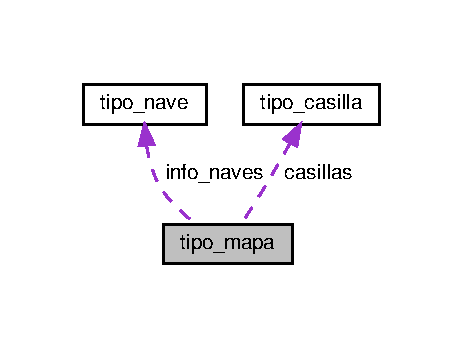
\includegraphics[width=222pt]{structtipo__mapa__coll__graph}
\end{center}
\end{figure}
\subsection*{Public Attributes}
\begin{DoxyCompactItemize}
\item 
\hyperlink{structtipo__nave}{tipo\+\_\+nave} \hyperlink{structtipo__mapa_a4796e19ff6b789ec44086b1bd662cd37}{info\+\_\+naves} \mbox{[}\hyperlink{simulador_8h_ab306668933fb4316ac0f5ef291d13dff}{N\+\_\+\+E\+Q\+U\+I\+P\+OS}\mbox{]}\mbox{[}\hyperlink{simulador_8h_aa1f2aba814c6d46772f9694849eeaa7a}{N\+\_\+\+N\+A\+V\+ES}\mbox{]}
\item 
\hyperlink{structtipo__casilla}{tipo\+\_\+casilla} \hyperlink{structtipo__mapa_a9fbe4aea60d084542050976284c2ea36}{casillas} \mbox{[}\hyperlink{simulador_8h_a5ae04aabcd69e10042a64a5dcf9a959d}{M\+A\+P\+A\+\_\+\+M\+A\+XY}\mbox{]}\mbox{[}\hyperlink{simulador_8h_ab55303c06ac5e3f77559983df0288e73}{M\+A\+P\+A\+\_\+\+M\+A\+XX}\mbox{]}
\item 
int \hyperlink{structtipo__mapa_a5a59bf5262122191c18e3a94eae24a8c}{num\+\_\+naves} \mbox{[}\hyperlink{simulador_8h_ab306668933fb4316ac0f5ef291d13dff}{N\+\_\+\+E\+Q\+U\+I\+P\+OS}\mbox{]}
\begin{DoxyCompactList}\small\item\em Número de naves vivas en un equipo. \end{DoxyCompactList}\item 
int \hyperlink{structtipo__mapa_a7f9e90d387d66f389630d65851398308}{contador\+Cola}
\item 
int \hyperlink{structtipo__mapa_a6cb20251f08713a0f1c08da2216d16e1}{contador\+Perdedores}
\end{DoxyCompactItemize}


\subsection{Detailed Description}
Estructura que almacena la informacion sobre el mapa. La estructura original proporcionada ha sido modificada para incluir un contador de los mensajes leidos y enviados por la cola de mensajes, y de los equipos que se vayan quedando sin naves. Esto facilita la reutilizacion de la zona de memoria compartida para el mapa, que permite utilizar estos nuevos campos sin necesidad de crear mas memoria compartida. 

\subsection{Member Data Documentation}
\mbox{\Hypertarget{structtipo__mapa_a9fbe4aea60d084542050976284c2ea36}\label{structtipo__mapa_a9fbe4aea60d084542050976284c2ea36}} 
\index{tipo\+\_\+mapa@{tipo\+\_\+mapa}!casillas@{casillas}}
\index{casillas@{casillas}!tipo\+\_\+mapa@{tipo\+\_\+mapa}}
\subsubsection{\texorpdfstring{casillas}{casillas}}
{\footnotesize\ttfamily \hyperlink{structtipo__casilla}{tipo\+\_\+casilla} tipo\+\_\+mapa\+::casillas\mbox{[}\hyperlink{simulador_8h_a5ae04aabcd69e10042a64a5dcf9a959d}{M\+A\+P\+A\+\_\+\+M\+A\+XY}\mbox{]}\mbox{[}\hyperlink{simulador_8h_ab55303c06ac5e3f77559983df0288e73}{M\+A\+P\+A\+\_\+\+M\+A\+XX}\mbox{]}}

\mbox{\Hypertarget{structtipo__mapa_a7f9e90d387d66f389630d65851398308}\label{structtipo__mapa_a7f9e90d387d66f389630d65851398308}} 
\index{tipo\+\_\+mapa@{tipo\+\_\+mapa}!contador\+Cola@{contador\+Cola}}
\index{contador\+Cola@{contador\+Cola}!tipo\+\_\+mapa@{tipo\+\_\+mapa}}
\subsubsection{\texorpdfstring{contador\+Cola}{contadorCola}}
{\footnotesize\ttfamily int tipo\+\_\+mapa\+::contador\+Cola}

\mbox{\Hypertarget{structtipo__mapa_a6cb20251f08713a0f1c08da2216d16e1}\label{structtipo__mapa_a6cb20251f08713a0f1c08da2216d16e1}} 
\index{tipo\+\_\+mapa@{tipo\+\_\+mapa}!contador\+Perdedores@{contador\+Perdedores}}
\index{contador\+Perdedores@{contador\+Perdedores}!tipo\+\_\+mapa@{tipo\+\_\+mapa}}
\subsubsection{\texorpdfstring{contador\+Perdedores}{contadorPerdedores}}
{\footnotesize\ttfamily int tipo\+\_\+mapa\+::contador\+Perdedores}

\mbox{\Hypertarget{structtipo__mapa_a4796e19ff6b789ec44086b1bd662cd37}\label{structtipo__mapa_a4796e19ff6b789ec44086b1bd662cd37}} 
\index{tipo\+\_\+mapa@{tipo\+\_\+mapa}!info\+\_\+naves@{info\+\_\+naves}}
\index{info\+\_\+naves@{info\+\_\+naves}!tipo\+\_\+mapa@{tipo\+\_\+mapa}}
\subsubsection{\texorpdfstring{info\+\_\+naves}{info\_naves}}
{\footnotesize\ttfamily \hyperlink{structtipo__nave}{tipo\+\_\+nave} tipo\+\_\+mapa\+::info\+\_\+naves\mbox{[}\hyperlink{simulador_8h_ab306668933fb4316ac0f5ef291d13dff}{N\+\_\+\+E\+Q\+U\+I\+P\+OS}\mbox{]}\mbox{[}\hyperlink{simulador_8h_aa1f2aba814c6d46772f9694849eeaa7a}{N\+\_\+\+N\+A\+V\+ES}\mbox{]}}

\mbox{\Hypertarget{structtipo__mapa_a5a59bf5262122191c18e3a94eae24a8c}\label{structtipo__mapa_a5a59bf5262122191c18e3a94eae24a8c}} 
\index{tipo\+\_\+mapa@{tipo\+\_\+mapa}!num\+\_\+naves@{num\+\_\+naves}}
\index{num\+\_\+naves@{num\+\_\+naves}!tipo\+\_\+mapa@{tipo\+\_\+mapa}}
\subsubsection{\texorpdfstring{num\+\_\+naves}{num\_naves}}
{\footnotesize\ttfamily int tipo\+\_\+mapa\+::num\+\_\+naves\mbox{[}\hyperlink{simulador_8h_ab306668933fb4316ac0f5ef291d13dff}{N\+\_\+\+E\+Q\+U\+I\+P\+OS}\mbox{]}}



Número de naves vivas en un equipo. 



The documentation for this struct was generated from the following file\+:\begin{DoxyCompactItemize}
\item 
src/\hyperlink{simulador_8h}{simulador.\+h}\end{DoxyCompactItemize}

\hypertarget{structtipo__nave}{}\section{tipo\+\_\+nave Struct Reference}
\label{structtipo__nave}\index{tipo\+\_\+nave@{tipo\+\_\+nave}}


Estructura que almacena la informacion sobre una nave.  




{\ttfamily \#include $<$simulador.\+h$>$}

\subsection*{Public Attributes}
\begin{DoxyCompactItemize}
\item 
int \hyperlink{structtipo__nave_a319f01d0152cadf2b976ef51c93ff7ae}{vida}
\begin{DoxyCompactList}\small\item\em Vida que le queda a la nave. \end{DoxyCompactList}\item 
int \hyperlink{structtipo__nave_a51b86c3dbe20a9fe15170f3660991fa4}{posx}
\begin{DoxyCompactList}\small\item\em Columna en el mapa. \end{DoxyCompactList}\item 
int \hyperlink{structtipo__nave_aecc547543a942bf2ae99356141bb436a}{posy}
\begin{DoxyCompactList}\small\item\em Fila en el mapa. \end{DoxyCompactList}\item 
int \hyperlink{structtipo__nave_a9cef996f47c2096f5ee3752c26adde97}{equipo}
\begin{DoxyCompactList}\small\item\em Equipo de la nave. \end{DoxyCompactList}\item 
int \hyperlink{structtipo__nave_a0184bdd515add385641c157beee1064c}{num\+Nave}
\begin{DoxyCompactList}\small\item\em Numero de la nave en el equipo. \end{DoxyCompactList}\item 
bool \hyperlink{structtipo__nave_a5fd530b54ff7694b07d41d3a168b800c}{viva}
\begin{DoxyCompactList}\small\item\em Si la nave está viva o ha sido destruida. \end{DoxyCompactList}\end{DoxyCompactItemize}


\subsection{Detailed Description}
Estructura que almacena la informacion sobre una nave. 

\subsection{Member Data Documentation}
\mbox{\Hypertarget{structtipo__nave_a9cef996f47c2096f5ee3752c26adde97}\label{structtipo__nave_a9cef996f47c2096f5ee3752c26adde97}} 
\index{tipo\+\_\+nave@{tipo\+\_\+nave}!equipo@{equipo}}
\index{equipo@{equipo}!tipo\+\_\+nave@{tipo\+\_\+nave}}
\subsubsection{\texorpdfstring{equipo}{equipo}}
{\footnotesize\ttfamily int tipo\+\_\+nave\+::equipo}



Equipo de la nave. 

\mbox{\Hypertarget{structtipo__nave_a0184bdd515add385641c157beee1064c}\label{structtipo__nave_a0184bdd515add385641c157beee1064c}} 
\index{tipo\+\_\+nave@{tipo\+\_\+nave}!num\+Nave@{num\+Nave}}
\index{num\+Nave@{num\+Nave}!tipo\+\_\+nave@{tipo\+\_\+nave}}
\subsubsection{\texorpdfstring{num\+Nave}{numNave}}
{\footnotesize\ttfamily int tipo\+\_\+nave\+::num\+Nave}



Numero de la nave en el equipo. 

\mbox{\Hypertarget{structtipo__nave_a51b86c3dbe20a9fe15170f3660991fa4}\label{structtipo__nave_a51b86c3dbe20a9fe15170f3660991fa4}} 
\index{tipo\+\_\+nave@{tipo\+\_\+nave}!posx@{posx}}
\index{posx@{posx}!tipo\+\_\+nave@{tipo\+\_\+nave}}
\subsubsection{\texorpdfstring{posx}{posx}}
{\footnotesize\ttfamily int tipo\+\_\+nave\+::posx}



Columna en el mapa. 

\mbox{\Hypertarget{structtipo__nave_aecc547543a942bf2ae99356141bb436a}\label{structtipo__nave_aecc547543a942bf2ae99356141bb436a}} 
\index{tipo\+\_\+nave@{tipo\+\_\+nave}!posy@{posy}}
\index{posy@{posy}!tipo\+\_\+nave@{tipo\+\_\+nave}}
\subsubsection{\texorpdfstring{posy}{posy}}
{\footnotesize\ttfamily int tipo\+\_\+nave\+::posy}



Fila en el mapa. 

\mbox{\Hypertarget{structtipo__nave_a319f01d0152cadf2b976ef51c93ff7ae}\label{structtipo__nave_a319f01d0152cadf2b976ef51c93ff7ae}} 
\index{tipo\+\_\+nave@{tipo\+\_\+nave}!vida@{vida}}
\index{vida@{vida}!tipo\+\_\+nave@{tipo\+\_\+nave}}
\subsubsection{\texorpdfstring{vida}{vida}}
{\footnotesize\ttfamily int tipo\+\_\+nave\+::vida}



Vida que le queda a la nave. 

\mbox{\Hypertarget{structtipo__nave_a5fd530b54ff7694b07d41d3a168b800c}\label{structtipo__nave_a5fd530b54ff7694b07d41d3a168b800c}} 
\index{tipo\+\_\+nave@{tipo\+\_\+nave}!viva@{viva}}
\index{viva@{viva}!tipo\+\_\+nave@{tipo\+\_\+nave}}
\subsubsection{\texorpdfstring{viva}{viva}}
{\footnotesize\ttfamily bool tipo\+\_\+nave\+::viva}



Si la nave está viva o ha sido destruida. 



The documentation for this struct was generated from the following file\+:\begin{DoxyCompactItemize}
\item 
src/\hyperlink{simulador_8h}{simulador.\+h}\end{DoxyCompactItemize}

\hypertarget{structTuberia}{}\section{Tuberia Struct Reference}
\label{structTuberia}\index{Tuberia@{Tuberia}}


Estructura que almacena tantos descriptores de ficheros como naves y jefes haya en la aplicacion. Se utilizara para inicializar las tuberias.  




{\ttfamily \#include $<$simulador.\+h$>$}

\subsection*{Public Attributes}
\begin{DoxyCompactItemize}
\item 
int \hyperlink{structTuberia_a14d4d7d33931e74e35ce8291fe944159}{fd} \mbox{[}\hyperlink{simulador_8h_ab306668933fb4316ac0f5ef291d13dff}{N\+\_\+\+E\+Q\+U\+I\+P\+OS}+(\hyperlink{simulador_8h_aa1f2aba814c6d46772f9694849eeaa7a}{N\+\_\+\+N\+A\+V\+ES} $\ast$\hyperlink{simulador_8h_ab306668933fb4316ac0f5ef291d13dff}{N\+\_\+\+E\+Q\+U\+I\+P\+OS})\mbox{]}\mbox{[}2\mbox{]}
\end{DoxyCompactItemize}


\subsection{Detailed Description}
Estructura que almacena tantos descriptores de ficheros como naves y jefes haya en la aplicacion. Se utilizara para inicializar las tuberias. 

\subsection{Member Data Documentation}
\mbox{\Hypertarget{structTuberia_a14d4d7d33931e74e35ce8291fe944159}\label{structTuberia_a14d4d7d33931e74e35ce8291fe944159}} 
\index{Tuberia@{Tuberia}!fd@{fd}}
\index{fd@{fd}!Tuberia@{Tuberia}}
\subsubsection{\texorpdfstring{fd}{fd}}
{\footnotesize\ttfamily int Tuberia\+::fd\mbox{[}\hyperlink{simulador_8h_ab306668933fb4316ac0f5ef291d13dff}{N\+\_\+\+E\+Q\+U\+I\+P\+OS}+(\hyperlink{simulador_8h_aa1f2aba814c6d46772f9694849eeaa7a}{N\+\_\+\+N\+A\+V\+ES} $\ast$\hyperlink{simulador_8h_ab306668933fb4316ac0f5ef291d13dff}{N\+\_\+\+E\+Q\+U\+I\+P\+OS})\mbox{]}\mbox{[}2\mbox{]}}



The documentation for this struct was generated from the following file\+:\begin{DoxyCompactItemize}
\item 
src/\hyperlink{simulador_8h}{simulador.\+h}\end{DoxyCompactItemize}

\chapter{File Documentation}
\hypertarget{gamescreen_8c}{}\section{src/gamescreen.c File Reference}
\label{gamescreen_8c}\index{src/gamescreen.\+c@{src/gamescreen.\+c}}
{\ttfamily \#include $<$ncurses.\+h$>$}\newline
Include dependency graph for gamescreen.\+c\+:
\nopagebreak
\begin{figure}[H]
\begin{center}
\leavevmode
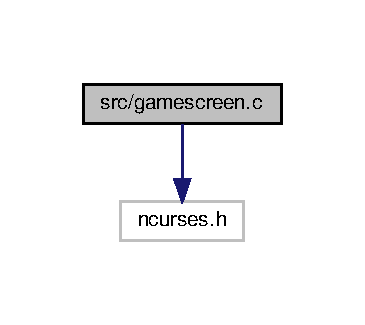
\includegraphics[width=175pt]{gamescreen_8c__incl}
\end{center}
\end{figure}
\subsection*{Functions}
\begin{DoxyCompactItemize}
\item 
void \hyperlink{gamescreen_8c_a9dbb6c251337c03c078dc330caee48d2}{screen\+\_\+init} ()
\item 
void \hyperlink{gamescreen_8c_a0780ee70c58765ba78d2c686dd14bd78}{screen\+\_\+addch} (int row, int col, char symbol)
\item 
void \hyperlink{gamescreen_8c_ab866ab906055d0fb46f4ccfa07c82173}{screen\+\_\+refresh} ()
\item 
void \hyperlink{gamescreen_8c_af3bc8be95518f1d57d6d201a980359be}{screen\+\_\+end} ()
\end{DoxyCompactItemize}


\subsection{Function Documentation}
\mbox{\Hypertarget{gamescreen_8c_a0780ee70c58765ba78d2c686dd14bd78}\label{gamescreen_8c_a0780ee70c58765ba78d2c686dd14bd78}} 
\index{gamescreen.\+c@{gamescreen.\+c}!screen\+\_\+addch@{screen\+\_\+addch}}
\index{screen\+\_\+addch@{screen\+\_\+addch}!gamescreen.\+c@{gamescreen.\+c}}
\subsubsection{\texorpdfstring{screen\+\_\+addch()}{screen\_addch()}}
{\footnotesize\ttfamily void screen\+\_\+addch (\begin{DoxyParamCaption}\item[{int}]{row,  }\item[{int}]{col,  }\item[{char}]{symbol }\end{DoxyParamCaption})}

\mbox{\Hypertarget{gamescreen_8c_af3bc8be95518f1d57d6d201a980359be}\label{gamescreen_8c_af3bc8be95518f1d57d6d201a980359be}} 
\index{gamescreen.\+c@{gamescreen.\+c}!screen\+\_\+end@{screen\+\_\+end}}
\index{screen\+\_\+end@{screen\+\_\+end}!gamescreen.\+c@{gamescreen.\+c}}
\subsubsection{\texorpdfstring{screen\+\_\+end()}{screen\_end()}}
{\footnotesize\ttfamily void screen\+\_\+end (\begin{DoxyParamCaption}{ }\end{DoxyParamCaption})}

\mbox{\Hypertarget{gamescreen_8c_a9dbb6c251337c03c078dc330caee48d2}\label{gamescreen_8c_a9dbb6c251337c03c078dc330caee48d2}} 
\index{gamescreen.\+c@{gamescreen.\+c}!screen\+\_\+init@{screen\+\_\+init}}
\index{screen\+\_\+init@{screen\+\_\+init}!gamescreen.\+c@{gamescreen.\+c}}
\subsubsection{\texorpdfstring{screen\+\_\+init()}{screen\_init()}}
{\footnotesize\ttfamily void screen\+\_\+init (\begin{DoxyParamCaption}{ }\end{DoxyParamCaption})}

\mbox{\Hypertarget{gamescreen_8c_ab866ab906055d0fb46f4ccfa07c82173}\label{gamescreen_8c_ab866ab906055d0fb46f4ccfa07c82173}} 
\index{gamescreen.\+c@{gamescreen.\+c}!screen\+\_\+refresh@{screen\+\_\+refresh}}
\index{screen\+\_\+refresh@{screen\+\_\+refresh}!gamescreen.\+c@{gamescreen.\+c}}
\subsubsection{\texorpdfstring{screen\+\_\+refresh()}{screen\_refresh()}}
{\footnotesize\ttfamily void screen\+\_\+refresh (\begin{DoxyParamCaption}{ }\end{DoxyParamCaption})}


\hypertarget{gamescreen_8h}{}\section{src/gamescreen.h File Reference}
\label{gamescreen_8h}\index{src/gamescreen.\+h@{src/gamescreen.\+h}}
This graph shows which files directly or indirectly include this file\+:
\nopagebreak
\begin{figure}[H]
\begin{center}
\leavevmode
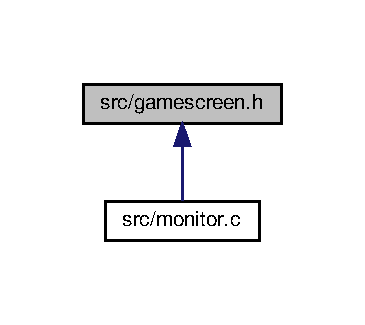
\includegraphics[width=175pt]{gamescreen_8h__dep__incl}
\end{center}
\end{figure}
\subsection*{Functions}
\begin{DoxyCompactItemize}
\item 
void \hyperlink{gamescreen_8h_a9dbb6c251337c03c078dc330caee48d2}{screen\+\_\+init} ()
\item 
void \hyperlink{gamescreen_8h_a0780ee70c58765ba78d2c686dd14bd78}{screen\+\_\+addch} (int row, int col, char symbol)
\item 
void \hyperlink{gamescreen_8h_ab866ab906055d0fb46f4ccfa07c82173}{screen\+\_\+refresh} ()
\item 
void \hyperlink{gamescreen_8h_af3bc8be95518f1d57d6d201a980359be}{screen\+\_\+end} ()
\end{DoxyCompactItemize}


\subsection{Function Documentation}
\mbox{\Hypertarget{gamescreen_8h_a0780ee70c58765ba78d2c686dd14bd78}\label{gamescreen_8h_a0780ee70c58765ba78d2c686dd14bd78}} 
\index{gamescreen.\+h@{gamescreen.\+h}!screen\+\_\+addch@{screen\+\_\+addch}}
\index{screen\+\_\+addch@{screen\+\_\+addch}!gamescreen.\+h@{gamescreen.\+h}}
\subsubsection{\texorpdfstring{screen\+\_\+addch()}{screen\_addch()}}
{\footnotesize\ttfamily void screen\+\_\+addch (\begin{DoxyParamCaption}\item[{int}]{row,  }\item[{int}]{col,  }\item[{char}]{symbol }\end{DoxyParamCaption})}

\mbox{\Hypertarget{gamescreen_8h_af3bc8be95518f1d57d6d201a980359be}\label{gamescreen_8h_af3bc8be95518f1d57d6d201a980359be}} 
\index{gamescreen.\+h@{gamescreen.\+h}!screen\+\_\+end@{screen\+\_\+end}}
\index{screen\+\_\+end@{screen\+\_\+end}!gamescreen.\+h@{gamescreen.\+h}}
\subsubsection{\texorpdfstring{screen\+\_\+end()}{screen\_end()}}
{\footnotesize\ttfamily void screen\+\_\+end (\begin{DoxyParamCaption}{ }\end{DoxyParamCaption})}

\mbox{\Hypertarget{gamescreen_8h_a9dbb6c251337c03c078dc330caee48d2}\label{gamescreen_8h_a9dbb6c251337c03c078dc330caee48d2}} 
\index{gamescreen.\+h@{gamescreen.\+h}!screen\+\_\+init@{screen\+\_\+init}}
\index{screen\+\_\+init@{screen\+\_\+init}!gamescreen.\+h@{gamescreen.\+h}}
\subsubsection{\texorpdfstring{screen\+\_\+init()}{screen\_init()}}
{\footnotesize\ttfamily void screen\+\_\+init (\begin{DoxyParamCaption}{ }\end{DoxyParamCaption})}

\mbox{\Hypertarget{gamescreen_8h_ab866ab906055d0fb46f4ccfa07c82173}\label{gamescreen_8h_ab866ab906055d0fb46f4ccfa07c82173}} 
\index{gamescreen.\+h@{gamescreen.\+h}!screen\+\_\+refresh@{screen\+\_\+refresh}}
\index{screen\+\_\+refresh@{screen\+\_\+refresh}!gamescreen.\+h@{gamescreen.\+h}}
\subsubsection{\texorpdfstring{screen\+\_\+refresh()}{screen\_refresh()}}
{\footnotesize\ttfamily void screen\+\_\+refresh (\begin{DoxyParamCaption}{ }\end{DoxyParamCaption})}


\hypertarget{jefe_8c}{}\section{src/jefe.c File Reference}
\label{jefe_8c}\index{src/jefe.\+c@{src/jefe.\+c}}


Programa que recibe ordenes del simulaodr y las procesa, decidiendo que ordenes enviar a las naves de manera aleatoria.  


{\ttfamily \#include $<$fcntl.\+h$>$}\newline
{\ttfamily \#include $<$sys/mman.\+h$>$}\newline
{\ttfamily \#include $<$sys/stat.\+h$>$}\newline
{\ttfamily \#include $<$sys/wait.\+h$>$}\newline
{\ttfamily \#include $<$stdio.\+h$>$}\newline
{\ttfamily \#include $<$stdlib.\+h$>$}\newline
{\ttfamily \#include $<$string.\+h$>$}\newline
{\ttfamily \#include $<$signal.\+h$>$}\newline
{\ttfamily \#include $<$math.\+h$>$}\newline
{\ttfamily \#include $<$stdbool.\+h$>$}\newline
{\ttfamily \#include $<$unistd.\+h$>$}\newline
{\ttfamily \#include $<$mapa.\+h$>$}\newline
{\ttfamily \#include $<$time.\+h$>$}\newline
{\ttfamily \#include $<$semaphore.\+h$>$}\newline
{\ttfamily \#include $<$simulador.\+h$>$}\newline
Include dependency graph for jefe.\+c\+:
\nopagebreak
\begin{figure}[H]
\begin{center}
\leavevmode
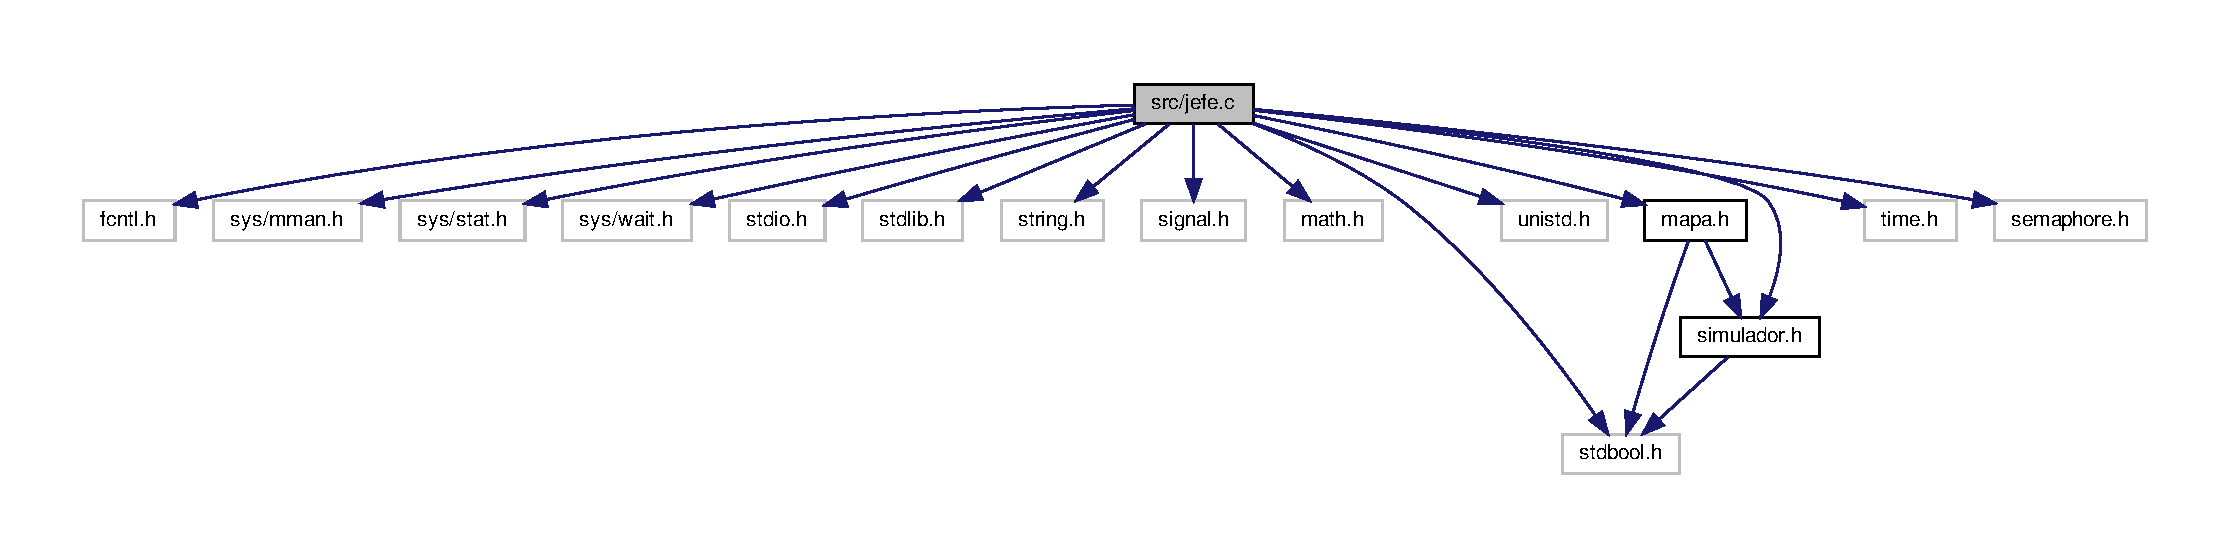
\includegraphics[width=350pt]{jefe_8c__incl}
\end{center}
\end{figure}
\subsection*{Macros}
\begin{DoxyCompactItemize}
\item 
\#define \hyperlink{jefe_8c_a24f3611c6828c8df80cb2b61dd3f1df4}{M\+Q\+\_\+\+N\+A\+ME}~\char`\"{}/mq\+\_\+nave\+Simulador\char`\"{}
\item 
\#define \hyperlink{jefe_8c_ad8e2b34b5877c257f4d561ceadc9e1c1}{S\+H\+M\+\_\+\+T\+UB}~\char`\"{}/shm\+\_\+tuberias\char`\"{}
\item 
\#define \hyperlink{jefe_8c_a86393b21e6f74e9870d92149e7fe7f20}{S\+H\+M\+\_\+\+N\+A\+ME}~\char`\"{}/shm\+\_\+estado\char`\"{}
\item 
\#define \hyperlink{jefe_8c_a486c681bc9fcbd82d87b80a479e6f72d}{S\+E\+M\+\_\+\+J\+E\+F\+ES}~\char`\"{}/sem\+\_\+jefes\char`\"{}
\end{DoxyCompactItemize}
\subsection*{Functions}
\begin{DoxyCompactItemize}
\item 
void \hyperlink{jefe_8c_a493ad48174879c61a0ed41fdffd829fa}{liberar} ()
\begin{DoxyCompactList}\small\item\em Funcion para liberar recursos. \end{DoxyCompactList}\item 
int \hyperlink{jefe_8c_abf9e6b7e6f15df4b525a2e7705ba3089}{main} (int argc, char const $\ast$argv\mbox{[}$\,$\mbox{]})
\end{DoxyCompactItemize}
\subsection*{Variables}
\begin{DoxyCompactItemize}
\item 
\hyperlink{structTuberia}{Tuberia} $\ast$ \hyperlink{jefe_8c_a677056758f5c7c430c4b6cb2543d138b}{tuberia}
\item 
int \hyperlink{jefe_8c_ab2944d7491ac51f8acc448d0a23f1da8}{memoria\+Tuberia}
\item 
sem\+\_\+t $\ast$ \hyperlink{jefe_8c_addb0adf902152934d52498fad43752e4}{sem\+\_\+jefes} = N\+U\+LL
\end{DoxyCompactItemize}


\subsection{Detailed Description}
Programa que recibe ordenes del simulaodr y las procesa, decidiendo que ordenes enviar a las naves de manera aleatoria. 

\begin{DoxyAuthor}{Author}
Alba Ramos\+: \href{mailto:alba.ramosp@estudiante.uam.es}{\tt alba.\+ramosp@estudiante.\+uam.\+es}; Grupo 2213 

Andrea Salcedo\+: \href{mailto:andrea.salcedo@estudiante.uam.es}{\tt andrea.\+salcedo@estudiante.\+uam.\+es}; Grupo 2213 
\end{DoxyAuthor}
\begin{DoxyDate}{Date}
11-\/04-\/2019 
\end{DoxyDate}


\subsection{Macro Definition Documentation}
\mbox{\Hypertarget{jefe_8c_a24f3611c6828c8df80cb2b61dd3f1df4}\label{jefe_8c_a24f3611c6828c8df80cb2b61dd3f1df4}} 
\index{jefe.\+c@{jefe.\+c}!M\+Q\+\_\+\+N\+A\+ME@{M\+Q\+\_\+\+N\+A\+ME}}
\index{M\+Q\+\_\+\+N\+A\+ME@{M\+Q\+\_\+\+N\+A\+ME}!jefe.\+c@{jefe.\+c}}
\subsubsection{\texorpdfstring{M\+Q\+\_\+\+N\+A\+ME}{MQ\_NAME}}
{\footnotesize\ttfamily \#define M\+Q\+\_\+\+N\+A\+ME~\char`\"{}/mq\+\_\+nave\+Simulador\char`\"{}}

\mbox{\Hypertarget{jefe_8c_a486c681bc9fcbd82d87b80a479e6f72d}\label{jefe_8c_a486c681bc9fcbd82d87b80a479e6f72d}} 
\index{jefe.\+c@{jefe.\+c}!S\+E\+M\+\_\+\+J\+E\+F\+ES@{S\+E\+M\+\_\+\+J\+E\+F\+ES}}
\index{S\+E\+M\+\_\+\+J\+E\+F\+ES@{S\+E\+M\+\_\+\+J\+E\+F\+ES}!jefe.\+c@{jefe.\+c}}
\subsubsection{\texorpdfstring{S\+E\+M\+\_\+\+J\+E\+F\+ES}{SEM\_JEFES}}
{\footnotesize\ttfamily \#define S\+E\+M\+\_\+\+J\+E\+F\+ES~\char`\"{}/sem\+\_\+jefes\char`\"{}}

\mbox{\Hypertarget{jefe_8c_a86393b21e6f74e9870d92149e7fe7f20}\label{jefe_8c_a86393b21e6f74e9870d92149e7fe7f20}} 
\index{jefe.\+c@{jefe.\+c}!S\+H\+M\+\_\+\+N\+A\+ME@{S\+H\+M\+\_\+\+N\+A\+ME}}
\index{S\+H\+M\+\_\+\+N\+A\+ME@{S\+H\+M\+\_\+\+N\+A\+ME}!jefe.\+c@{jefe.\+c}}
\subsubsection{\texorpdfstring{S\+H\+M\+\_\+\+N\+A\+ME}{SHM\_NAME}}
{\footnotesize\ttfamily \#define S\+H\+M\+\_\+\+N\+A\+ME~\char`\"{}/shm\+\_\+estado\char`\"{}}

\mbox{\Hypertarget{jefe_8c_ad8e2b34b5877c257f4d561ceadc9e1c1}\label{jefe_8c_ad8e2b34b5877c257f4d561ceadc9e1c1}} 
\index{jefe.\+c@{jefe.\+c}!S\+H\+M\+\_\+\+T\+UB@{S\+H\+M\+\_\+\+T\+UB}}
\index{S\+H\+M\+\_\+\+T\+UB@{S\+H\+M\+\_\+\+T\+UB}!jefe.\+c@{jefe.\+c}}
\subsubsection{\texorpdfstring{S\+H\+M\+\_\+\+T\+UB}{SHM\_TUB}}
{\footnotesize\ttfamily \#define S\+H\+M\+\_\+\+T\+UB~\char`\"{}/shm\+\_\+tuberias\char`\"{}}



\subsection{Function Documentation}
\mbox{\Hypertarget{jefe_8c_a493ad48174879c61a0ed41fdffd829fa}\label{jefe_8c_a493ad48174879c61a0ed41fdffd829fa}} 
\index{jefe.\+c@{jefe.\+c}!liberar@{liberar}}
\index{liberar@{liberar}!jefe.\+c@{jefe.\+c}}
\subsubsection{\texorpdfstring{liberar()}{liberar()}}
{\footnotesize\ttfamily void liberar (\begin{DoxyParamCaption}{ }\end{DoxyParamCaption})}



Funcion para liberar recursos. 

\begin{DoxyReturn}{Returns}
void 
\end{DoxyReturn}
\mbox{\Hypertarget{jefe_8c_abf9e6b7e6f15df4b525a2e7705ba3089}\label{jefe_8c_abf9e6b7e6f15df4b525a2e7705ba3089}} 
\index{jefe.\+c@{jefe.\+c}!main@{main}}
\index{main@{main}!jefe.\+c@{jefe.\+c}}
\subsubsection{\texorpdfstring{main()}{main()}}
{\footnotesize\ttfamily int main (\begin{DoxyParamCaption}\item[{int}]{argc,  }\item[{char const $\ast$}]{argv\mbox{[}$\,$\mbox{]} }\end{DoxyParamCaption})}



\subsection{Variable Documentation}
\mbox{\Hypertarget{jefe_8c_ab2944d7491ac51f8acc448d0a23f1da8}\label{jefe_8c_ab2944d7491ac51f8acc448d0a23f1da8}} 
\index{jefe.\+c@{jefe.\+c}!memoria\+Tuberia@{memoria\+Tuberia}}
\index{memoria\+Tuberia@{memoria\+Tuberia}!jefe.\+c@{jefe.\+c}}
\subsubsection{\texorpdfstring{memoria\+Tuberia}{memoriaTuberia}}
{\footnotesize\ttfamily int memoria\+Tuberia}

Memoria compartida para almacenar la tuberia \mbox{\Hypertarget{jefe_8c_addb0adf902152934d52498fad43752e4}\label{jefe_8c_addb0adf902152934d52498fad43752e4}} 
\index{jefe.\+c@{jefe.\+c}!sem\+\_\+jefes@{sem\+\_\+jefes}}
\index{sem\+\_\+jefes@{sem\+\_\+jefes}!jefe.\+c@{jefe.\+c}}
\subsubsection{\texorpdfstring{sem\+\_\+jefes}{sem\_jefes}}
{\footnotesize\ttfamily sem\+\_\+t$\ast$ sem\+\_\+jefes = N\+U\+LL}

Semaforo para indicar que el jefe ha esperado a que todas las naves esten creadas \mbox{\Hypertarget{jefe_8c_a677056758f5c7c430c4b6cb2543d138b}\label{jefe_8c_a677056758f5c7c430c4b6cb2543d138b}} 
\index{jefe.\+c@{jefe.\+c}!tuberia@{tuberia}}
\index{tuberia@{tuberia}!jefe.\+c@{jefe.\+c}}
\subsubsection{\texorpdfstring{tuberia}{tuberia}}
{\footnotesize\ttfamily \hyperlink{structTuberia}{Tuberia}$\ast$ tuberia}

\hyperlink{structTuberia}{Tuberia} para recibir los mensajes del simulador 
\hypertarget{mapa_8c}{}\section{src/mapa.c File Reference}
\label{mapa_8c}\index{src/mapa.\+c@{src/mapa.\+c}}
{\ttfamily \#include \char`\"{}mapa.\+h\char`\"{}}\newline
{\ttfamily \#include $<$stdbool.\+h$>$}\newline
{\ttfamily \#include $<$math.\+h$>$}\newline
{\ttfamily \#include $<$stdlib.\+h$>$}\newline
{\ttfamily \#include $<$unistd.\+h$>$}\newline
{\ttfamily \#include $<$stdio.\+h$>$}\newline
Include dependency graph for mapa.\+c\+:
\nopagebreak
\begin{figure}[H]
\begin{center}
\leavevmode
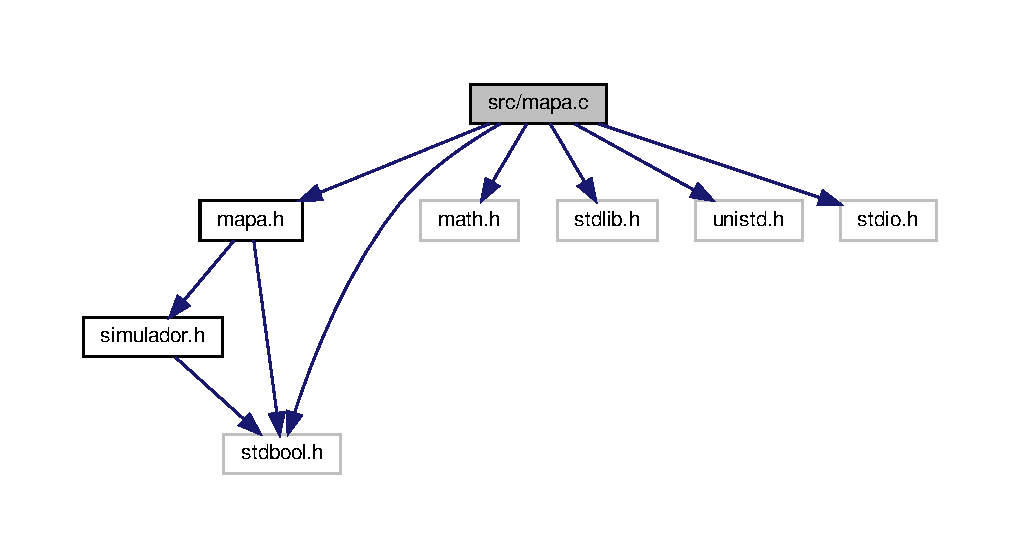
\includegraphics[width=350pt]{mapa_8c__incl}
\end{center}
\end{figure}
\subsection*{Functions}
\begin{DoxyCompactItemize}
\item 
int \hyperlink{mapa_8c_ae3d2270d9e93086430a1e5cf639aab53}{mapa\+\_\+clean\+\_\+casilla} (\hyperlink{structtipo__mapa}{tipo\+\_\+mapa} $\ast$\hyperlink{simulador_8c_a3f88248411450095465da3e38eb812c2}{mapa}, int posy, int posx)
\item 
\hyperlink{structtipo__casilla}{tipo\+\_\+casilla} \hyperlink{mapa_8c_adedc40364bffd27208a7287434c28c15}{mapa\+\_\+get\+\_\+casilla} (\hyperlink{structtipo__mapa}{tipo\+\_\+mapa} $\ast$\hyperlink{simulador_8c_a3f88248411450095465da3e38eb812c2}{mapa}, int posy, int posx)
\item 
int \hyperlink{mapa_8c_a356da64c56ecdaddca0ab55794efd8b1}{mapa\+\_\+get\+\_\+distancia} (\hyperlink{structtipo__mapa}{tipo\+\_\+mapa} $\ast$\hyperlink{simulador_8c_a3f88248411450095465da3e38eb812c2}{mapa}, int oriy, int orix, int targety, int targetx)
\item 
\hyperlink{structtipo__nave}{tipo\+\_\+nave} \hyperlink{mapa_8c_ae949a08280aeec8b57b32906b6d73f78}{mapa\+\_\+get\+\_\+nave} (\hyperlink{structtipo__mapa}{tipo\+\_\+mapa} $\ast$\hyperlink{simulador_8c_a3f88248411450095465da3e38eb812c2}{mapa}, int \hyperlink{nave_8c_aa5e6716194f228a7cc36e89f613a30d0}{equipo}, int num\+\_\+nave)
\item 
int \hyperlink{mapa_8c_a407e4361ece24cdd19cb0070181fbb91}{mapa\+\_\+get\+\_\+num\+\_\+naves} (\hyperlink{structtipo__mapa}{tipo\+\_\+mapa} $\ast$\hyperlink{simulador_8c_a3f88248411450095465da3e38eb812c2}{mapa}, int \hyperlink{nave_8c_aa5e6716194f228a7cc36e89f613a30d0}{equipo})
\item 
char \hyperlink{mapa_8c_a264d3cdb7ec0b8f335adeddae138edb3}{mapa\+\_\+get\+\_\+symbol} (\hyperlink{structtipo__mapa}{tipo\+\_\+mapa} $\ast$\hyperlink{simulador_8c_a3f88248411450095465da3e38eb812c2}{mapa}, int posy, int posx)
\item 
bool \hyperlink{mapa_8c_a23a5362da8e4c482a8300fad3e25701c}{mapa\+\_\+is\+\_\+casilla\+\_\+vacia} (\hyperlink{structtipo__mapa}{tipo\+\_\+mapa} $\ast$\hyperlink{simulador_8c_a3f88248411450095465da3e38eb812c2}{mapa}, int posy, int posx)
\item 
void \hyperlink{mapa_8c_a555fccad30331311a6185a03c4a53f64}{mapa\+\_\+restore} (\hyperlink{structtipo__mapa}{tipo\+\_\+mapa} $\ast$\hyperlink{simulador_8c_a3f88248411450095465da3e38eb812c2}{mapa})
\item 
void \hyperlink{mapa_8c_a785183133f1f9d50fa6445d4245610aa}{mapa\+\_\+set\+\_\+symbol} (\hyperlink{structtipo__mapa}{tipo\+\_\+mapa} $\ast$\hyperlink{simulador_8c_a3f88248411450095465da3e38eb812c2}{mapa}, int posy, int posx, char symbol)
\item 
int \hyperlink{mapa_8c_a9ffafdce1656b32f99897e5395cf3e04}{mapa\+\_\+set\+\_\+nave} (\hyperlink{structtipo__mapa}{tipo\+\_\+mapa} $\ast$\hyperlink{simulador_8c_a3f88248411450095465da3e38eb812c2}{mapa}, \hyperlink{structtipo__nave}{tipo\+\_\+nave} nave)
\item 
void \hyperlink{mapa_8c_a402d2eed071e74def79173a09a207745}{mapa\+\_\+set\+\_\+num\+\_\+naves} (\hyperlink{structtipo__mapa}{tipo\+\_\+mapa} $\ast$\hyperlink{simulador_8c_a3f88248411450095465da3e38eb812c2}{mapa}, int \hyperlink{nave_8c_aa5e6716194f228a7cc36e89f613a30d0}{equipo}, int num\+Naves)
\item 
void \hyperlink{mapa_8c_a21f4b84a16bcf27cf4ba48a8aa523cbd}{mapa\+\_\+send\+\_\+misil} (\hyperlink{structtipo__mapa}{tipo\+\_\+mapa} $\ast$\hyperlink{simulador_8c_a3f88248411450095465da3e38eb812c2}{mapa}, int origeny, int origenx, int targety, int targetx)
\end{DoxyCompactItemize}
\subsection*{Variables}
\begin{DoxyCompactItemize}
\item 
char \hyperlink{mapa_8c_a8aa1e6a79521de10e22a0a7574f2c8a5}{symbol\+\_\+equipos} \mbox{[}\hyperlink{simulador_8h_ab306668933fb4316ac0f5ef291d13dff}{N\+\_\+\+E\+Q\+U\+I\+P\+OS}\mbox{]} =\{\textquotesingle{}A\textquotesingle{},\textquotesingle{}B\textquotesingle{},\textquotesingle{}C\textquotesingle{}\}
\end{DoxyCompactItemize}


\subsection{Function Documentation}
\mbox{\Hypertarget{mapa_8c_ae3d2270d9e93086430a1e5cf639aab53}\label{mapa_8c_ae3d2270d9e93086430a1e5cf639aab53}} 
\index{mapa.\+c@{mapa.\+c}!mapa\+\_\+clean\+\_\+casilla@{mapa\+\_\+clean\+\_\+casilla}}
\index{mapa\+\_\+clean\+\_\+casilla@{mapa\+\_\+clean\+\_\+casilla}!mapa.\+c@{mapa.\+c}}
\subsubsection{\texorpdfstring{mapa\+\_\+clean\+\_\+casilla()}{mapa\_clean\_casilla()}}
{\footnotesize\ttfamily int mapa\+\_\+clean\+\_\+casilla (\begin{DoxyParamCaption}\item[{\hyperlink{structtipo__mapa}{tipo\+\_\+mapa} $\ast$}]{mapa,  }\item[{int}]{posy,  }\item[{int}]{posx }\end{DoxyParamCaption})}

\mbox{\Hypertarget{mapa_8c_adedc40364bffd27208a7287434c28c15}\label{mapa_8c_adedc40364bffd27208a7287434c28c15}} 
\index{mapa.\+c@{mapa.\+c}!mapa\+\_\+get\+\_\+casilla@{mapa\+\_\+get\+\_\+casilla}}
\index{mapa\+\_\+get\+\_\+casilla@{mapa\+\_\+get\+\_\+casilla}!mapa.\+c@{mapa.\+c}}
\subsubsection{\texorpdfstring{mapa\+\_\+get\+\_\+casilla()}{mapa\_get\_casilla()}}
{\footnotesize\ttfamily \hyperlink{structtipo__casilla}{tipo\+\_\+casilla} mapa\+\_\+get\+\_\+casilla (\begin{DoxyParamCaption}\item[{\hyperlink{structtipo__mapa}{tipo\+\_\+mapa} $\ast$}]{mapa,  }\item[{int}]{posy,  }\item[{int}]{posx }\end{DoxyParamCaption})}

\mbox{\Hypertarget{mapa_8c_a356da64c56ecdaddca0ab55794efd8b1}\label{mapa_8c_a356da64c56ecdaddca0ab55794efd8b1}} 
\index{mapa.\+c@{mapa.\+c}!mapa\+\_\+get\+\_\+distancia@{mapa\+\_\+get\+\_\+distancia}}
\index{mapa\+\_\+get\+\_\+distancia@{mapa\+\_\+get\+\_\+distancia}!mapa.\+c@{mapa.\+c}}
\subsubsection{\texorpdfstring{mapa\+\_\+get\+\_\+distancia()}{mapa\_get\_distancia()}}
{\footnotesize\ttfamily int mapa\+\_\+get\+\_\+distancia (\begin{DoxyParamCaption}\item[{\hyperlink{structtipo__mapa}{tipo\+\_\+mapa} $\ast$}]{mapa,  }\item[{int}]{oriy,  }\item[{int}]{orix,  }\item[{int}]{targety,  }\item[{int}]{targetx }\end{DoxyParamCaption})}

\mbox{\Hypertarget{mapa_8c_ae949a08280aeec8b57b32906b6d73f78}\label{mapa_8c_ae949a08280aeec8b57b32906b6d73f78}} 
\index{mapa.\+c@{mapa.\+c}!mapa\+\_\+get\+\_\+nave@{mapa\+\_\+get\+\_\+nave}}
\index{mapa\+\_\+get\+\_\+nave@{mapa\+\_\+get\+\_\+nave}!mapa.\+c@{mapa.\+c}}
\subsubsection{\texorpdfstring{mapa\+\_\+get\+\_\+nave()}{mapa\_get\_nave()}}
{\footnotesize\ttfamily \hyperlink{structtipo__nave}{tipo\+\_\+nave} mapa\+\_\+get\+\_\+nave (\begin{DoxyParamCaption}\item[{\hyperlink{structtipo__mapa}{tipo\+\_\+mapa} $\ast$}]{mapa,  }\item[{int}]{equipo,  }\item[{int}]{num\+\_\+nave }\end{DoxyParamCaption})}

\mbox{\Hypertarget{mapa_8c_a407e4361ece24cdd19cb0070181fbb91}\label{mapa_8c_a407e4361ece24cdd19cb0070181fbb91}} 
\index{mapa.\+c@{mapa.\+c}!mapa\+\_\+get\+\_\+num\+\_\+naves@{mapa\+\_\+get\+\_\+num\+\_\+naves}}
\index{mapa\+\_\+get\+\_\+num\+\_\+naves@{mapa\+\_\+get\+\_\+num\+\_\+naves}!mapa.\+c@{mapa.\+c}}
\subsubsection{\texorpdfstring{mapa\+\_\+get\+\_\+num\+\_\+naves()}{mapa\_get\_num\_naves()}}
{\footnotesize\ttfamily int mapa\+\_\+get\+\_\+num\+\_\+naves (\begin{DoxyParamCaption}\item[{\hyperlink{structtipo__mapa}{tipo\+\_\+mapa} $\ast$}]{mapa,  }\item[{int}]{equipo }\end{DoxyParamCaption})}

\mbox{\Hypertarget{mapa_8c_a264d3cdb7ec0b8f335adeddae138edb3}\label{mapa_8c_a264d3cdb7ec0b8f335adeddae138edb3}} 
\index{mapa.\+c@{mapa.\+c}!mapa\+\_\+get\+\_\+symbol@{mapa\+\_\+get\+\_\+symbol}}
\index{mapa\+\_\+get\+\_\+symbol@{mapa\+\_\+get\+\_\+symbol}!mapa.\+c@{mapa.\+c}}
\subsubsection{\texorpdfstring{mapa\+\_\+get\+\_\+symbol()}{mapa\_get\_symbol()}}
{\footnotesize\ttfamily char mapa\+\_\+get\+\_\+symbol (\begin{DoxyParamCaption}\item[{\hyperlink{structtipo__mapa}{tipo\+\_\+mapa} $\ast$}]{mapa,  }\item[{int}]{posy,  }\item[{int}]{posx }\end{DoxyParamCaption})}

\mbox{\Hypertarget{mapa_8c_a23a5362da8e4c482a8300fad3e25701c}\label{mapa_8c_a23a5362da8e4c482a8300fad3e25701c}} 
\index{mapa.\+c@{mapa.\+c}!mapa\+\_\+is\+\_\+casilla\+\_\+vacia@{mapa\+\_\+is\+\_\+casilla\+\_\+vacia}}
\index{mapa\+\_\+is\+\_\+casilla\+\_\+vacia@{mapa\+\_\+is\+\_\+casilla\+\_\+vacia}!mapa.\+c@{mapa.\+c}}
\subsubsection{\texorpdfstring{mapa\+\_\+is\+\_\+casilla\+\_\+vacia()}{mapa\_is\_casilla\_vacia()}}
{\footnotesize\ttfamily bool mapa\+\_\+is\+\_\+casilla\+\_\+vacia (\begin{DoxyParamCaption}\item[{\hyperlink{structtipo__mapa}{tipo\+\_\+mapa} $\ast$}]{mapa,  }\item[{int}]{posy,  }\item[{int}]{posx }\end{DoxyParamCaption})}

\mbox{\Hypertarget{mapa_8c_a555fccad30331311a6185a03c4a53f64}\label{mapa_8c_a555fccad30331311a6185a03c4a53f64}} 
\index{mapa.\+c@{mapa.\+c}!mapa\+\_\+restore@{mapa\+\_\+restore}}
\index{mapa\+\_\+restore@{mapa\+\_\+restore}!mapa.\+c@{mapa.\+c}}
\subsubsection{\texorpdfstring{mapa\+\_\+restore()}{mapa\_restore()}}
{\footnotesize\ttfamily void mapa\+\_\+restore (\begin{DoxyParamCaption}\item[{\hyperlink{structtipo__mapa}{tipo\+\_\+mapa} $\ast$}]{mapa }\end{DoxyParamCaption})}

\mbox{\Hypertarget{mapa_8c_a21f4b84a16bcf27cf4ba48a8aa523cbd}\label{mapa_8c_a21f4b84a16bcf27cf4ba48a8aa523cbd}} 
\index{mapa.\+c@{mapa.\+c}!mapa\+\_\+send\+\_\+misil@{mapa\+\_\+send\+\_\+misil}}
\index{mapa\+\_\+send\+\_\+misil@{mapa\+\_\+send\+\_\+misil}!mapa.\+c@{mapa.\+c}}
\subsubsection{\texorpdfstring{mapa\+\_\+send\+\_\+misil()}{mapa\_send\_misil()}}
{\footnotesize\ttfamily void mapa\+\_\+send\+\_\+misil (\begin{DoxyParamCaption}\item[{\hyperlink{structtipo__mapa}{tipo\+\_\+mapa} $\ast$}]{mapa,  }\item[{int}]{origeny,  }\item[{int}]{origenx,  }\item[{int}]{targety,  }\item[{int}]{targetx }\end{DoxyParamCaption})}

\mbox{\Hypertarget{mapa_8c_a9ffafdce1656b32f99897e5395cf3e04}\label{mapa_8c_a9ffafdce1656b32f99897e5395cf3e04}} 
\index{mapa.\+c@{mapa.\+c}!mapa\+\_\+set\+\_\+nave@{mapa\+\_\+set\+\_\+nave}}
\index{mapa\+\_\+set\+\_\+nave@{mapa\+\_\+set\+\_\+nave}!mapa.\+c@{mapa.\+c}}
\subsubsection{\texorpdfstring{mapa\+\_\+set\+\_\+nave()}{mapa\_set\_nave()}}
{\footnotesize\ttfamily int mapa\+\_\+set\+\_\+nave (\begin{DoxyParamCaption}\item[{\hyperlink{structtipo__mapa}{tipo\+\_\+mapa} $\ast$}]{mapa,  }\item[{\hyperlink{structtipo__nave}{tipo\+\_\+nave}}]{nave }\end{DoxyParamCaption})}

\mbox{\Hypertarget{mapa_8c_a402d2eed071e74def79173a09a207745}\label{mapa_8c_a402d2eed071e74def79173a09a207745}} 
\index{mapa.\+c@{mapa.\+c}!mapa\+\_\+set\+\_\+num\+\_\+naves@{mapa\+\_\+set\+\_\+num\+\_\+naves}}
\index{mapa\+\_\+set\+\_\+num\+\_\+naves@{mapa\+\_\+set\+\_\+num\+\_\+naves}!mapa.\+c@{mapa.\+c}}
\subsubsection{\texorpdfstring{mapa\+\_\+set\+\_\+num\+\_\+naves()}{mapa\_set\_num\_naves()}}
{\footnotesize\ttfamily void mapa\+\_\+set\+\_\+num\+\_\+naves (\begin{DoxyParamCaption}\item[{\hyperlink{structtipo__mapa}{tipo\+\_\+mapa} $\ast$}]{mapa,  }\item[{int}]{equipo,  }\item[{int}]{num\+Naves }\end{DoxyParamCaption})}

\mbox{\Hypertarget{mapa_8c_a785183133f1f9d50fa6445d4245610aa}\label{mapa_8c_a785183133f1f9d50fa6445d4245610aa}} 
\index{mapa.\+c@{mapa.\+c}!mapa\+\_\+set\+\_\+symbol@{mapa\+\_\+set\+\_\+symbol}}
\index{mapa\+\_\+set\+\_\+symbol@{mapa\+\_\+set\+\_\+symbol}!mapa.\+c@{mapa.\+c}}
\subsubsection{\texorpdfstring{mapa\+\_\+set\+\_\+symbol()}{mapa\_set\_symbol()}}
{\footnotesize\ttfamily void mapa\+\_\+set\+\_\+symbol (\begin{DoxyParamCaption}\item[{\hyperlink{structtipo__mapa}{tipo\+\_\+mapa} $\ast$}]{mapa,  }\item[{int}]{posy,  }\item[{int}]{posx,  }\item[{char}]{symbol }\end{DoxyParamCaption})}



\subsection{Variable Documentation}
\mbox{\Hypertarget{mapa_8c_a8aa1e6a79521de10e22a0a7574f2c8a5}\label{mapa_8c_a8aa1e6a79521de10e22a0a7574f2c8a5}} 
\index{mapa.\+c@{mapa.\+c}!symbol\+\_\+equipos@{symbol\+\_\+equipos}}
\index{symbol\+\_\+equipos@{symbol\+\_\+equipos}!mapa.\+c@{mapa.\+c}}
\subsubsection{\texorpdfstring{symbol\+\_\+equipos}{symbol\_equipos}}
{\footnotesize\ttfamily char symbol\+\_\+equipos\mbox{[}\hyperlink{simulador_8h_ab306668933fb4316ac0f5ef291d13dff}{N\+\_\+\+E\+Q\+U\+I\+P\+OS}\mbox{]} =\{\textquotesingle{}A\textquotesingle{},\textquotesingle{}B\textquotesingle{},\textquotesingle{}C\textquotesingle{}\}}

Símbolos de los diferentes equipos en el mapa (mirar \hyperlink{mapa_8c}{mapa.\+c}) 
\hypertarget{mapa_8h}{}\section{src/mapa.h File Reference}
\label{mapa_8h}\index{src/mapa.\+h@{src/mapa.\+h}}
{\ttfamily \#include $<$simulador.\+h$>$}\newline
{\ttfamily \#include $<$stdbool.\+h$>$}\newline
Include dependency graph for mapa.\+h\+:
\nopagebreak
\begin{figure}[H]
\begin{center}
\leavevmode
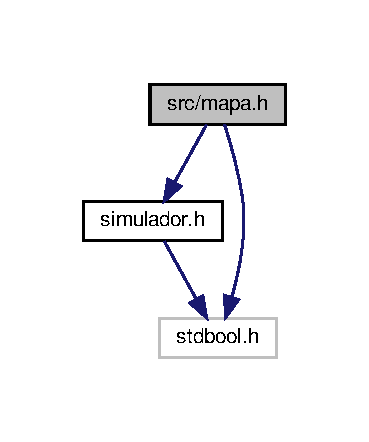
\includegraphics[width=177pt]{mapa_8h__incl}
\end{center}
\end{figure}
This graph shows which files directly or indirectly include this file\+:
\nopagebreak
\begin{figure}[H]
\begin{center}
\leavevmode
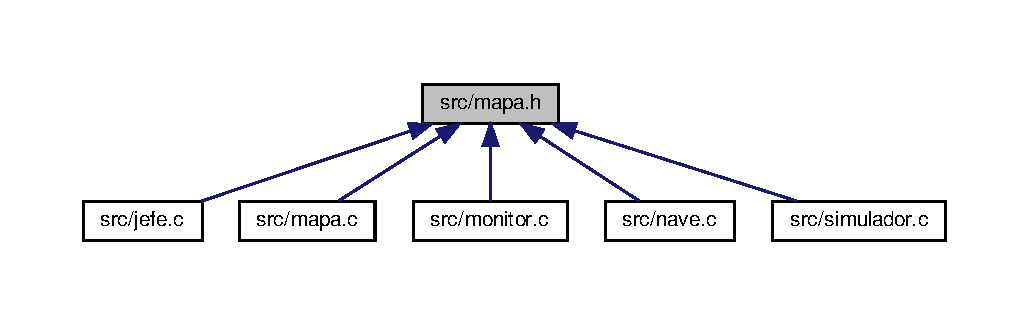
\includegraphics[width=350pt]{mapa_8h__dep__incl}
\end{center}
\end{figure}
\subsection*{Functions}
\begin{DoxyCompactItemize}
\item 
int \hyperlink{mapa_8h_ae3d2270d9e93086430a1e5cf639aab53}{mapa\+\_\+clean\+\_\+casilla} (\hyperlink{structtipo__mapa}{tipo\+\_\+mapa} $\ast$\hyperlink{simulador_8c_a3f88248411450095465da3e38eb812c2}{mapa}, int posy, int posx)
\item 
\hyperlink{structtipo__casilla}{tipo\+\_\+casilla} \hyperlink{mapa_8h_adedc40364bffd27208a7287434c28c15}{mapa\+\_\+get\+\_\+casilla} (\hyperlink{structtipo__mapa}{tipo\+\_\+mapa} $\ast$\hyperlink{simulador_8c_a3f88248411450095465da3e38eb812c2}{mapa}, int posy, int posx)
\item 
int \hyperlink{mapa_8h_a356da64c56ecdaddca0ab55794efd8b1}{mapa\+\_\+get\+\_\+distancia} (\hyperlink{structtipo__mapa}{tipo\+\_\+mapa} $\ast$\hyperlink{simulador_8c_a3f88248411450095465da3e38eb812c2}{mapa}, int oriy, int orix, int targety, int targetx)
\item 
\hyperlink{structtipo__nave}{tipo\+\_\+nave} \hyperlink{mapa_8h_ae949a08280aeec8b57b32906b6d73f78}{mapa\+\_\+get\+\_\+nave} (\hyperlink{structtipo__mapa}{tipo\+\_\+mapa} $\ast$\hyperlink{simulador_8c_a3f88248411450095465da3e38eb812c2}{mapa}, int \hyperlink{nave_8c_aa5e6716194f228a7cc36e89f613a30d0}{equipo}, int num\+\_\+nave)
\item 
int \hyperlink{mapa_8h_a407e4361ece24cdd19cb0070181fbb91}{mapa\+\_\+get\+\_\+num\+\_\+naves} (\hyperlink{structtipo__mapa}{tipo\+\_\+mapa} $\ast$\hyperlink{simulador_8c_a3f88248411450095465da3e38eb812c2}{mapa}, int \hyperlink{nave_8c_aa5e6716194f228a7cc36e89f613a30d0}{equipo})
\item 
char \hyperlink{mapa_8h_a264d3cdb7ec0b8f335adeddae138edb3}{mapa\+\_\+get\+\_\+symbol} (\hyperlink{structtipo__mapa}{tipo\+\_\+mapa} $\ast$\hyperlink{simulador_8c_a3f88248411450095465da3e38eb812c2}{mapa}, int posy, int posx)
\item 
bool \hyperlink{mapa_8h_a23a5362da8e4c482a8300fad3e25701c}{mapa\+\_\+is\+\_\+casilla\+\_\+vacia} (\hyperlink{structtipo__mapa}{tipo\+\_\+mapa} $\ast$\hyperlink{simulador_8c_a3f88248411450095465da3e38eb812c2}{mapa}, int posy, int posx)
\item 
bool \hyperlink{mapa_8h_a5a9cdda0532af3135bd8530819f58915}{casilla\+\_\+is\+\_\+vacia} (\hyperlink{structtipo__mapa}{tipo\+\_\+mapa} $\ast$\hyperlink{simulador_8c_a3f88248411450095465da3e38eb812c2}{mapa}, \hyperlink{structtipo__casilla}{tipo\+\_\+casilla} casilla)
\item 
void \hyperlink{mapa_8h_a555fccad30331311a6185a03c4a53f64}{mapa\+\_\+restore} (\hyperlink{structtipo__mapa}{tipo\+\_\+mapa} $\ast$\hyperlink{simulador_8c_a3f88248411450095465da3e38eb812c2}{mapa})
\item 
void \hyperlink{mapa_8h_a21f4b84a16bcf27cf4ba48a8aa523cbd}{mapa\+\_\+send\+\_\+misil} (\hyperlink{structtipo__mapa}{tipo\+\_\+mapa} $\ast$\hyperlink{simulador_8c_a3f88248411450095465da3e38eb812c2}{mapa}, int origeny, int origenx, int targety, int targetx)
\item 
int \hyperlink{mapa_8h_a9ffafdce1656b32f99897e5395cf3e04}{mapa\+\_\+set\+\_\+nave} (\hyperlink{structtipo__mapa}{tipo\+\_\+mapa} $\ast$\hyperlink{simulador_8c_a3f88248411450095465da3e38eb812c2}{mapa}, \hyperlink{structtipo__nave}{tipo\+\_\+nave} nave)
\item 
void \hyperlink{mapa_8h_a402d2eed071e74def79173a09a207745}{mapa\+\_\+set\+\_\+num\+\_\+naves} (\hyperlink{structtipo__mapa}{tipo\+\_\+mapa} $\ast$\hyperlink{simulador_8c_a3f88248411450095465da3e38eb812c2}{mapa}, int \hyperlink{nave_8c_aa5e6716194f228a7cc36e89f613a30d0}{equipo}, int num\+Naves)
\item 
void \hyperlink{mapa_8h_a785183133f1f9d50fa6445d4245610aa}{mapa\+\_\+set\+\_\+symbol} (\hyperlink{structtipo__mapa}{tipo\+\_\+mapa} $\ast$\hyperlink{simulador_8c_a3f88248411450095465da3e38eb812c2}{mapa}, int posy, int posx, char symbol)
\end{DoxyCompactItemize}


\subsection{Function Documentation}
\mbox{\Hypertarget{mapa_8h_a5a9cdda0532af3135bd8530819f58915}\label{mapa_8h_a5a9cdda0532af3135bd8530819f58915}} 
\index{mapa.\+h@{mapa.\+h}!casilla\+\_\+is\+\_\+vacia@{casilla\+\_\+is\+\_\+vacia}}
\index{casilla\+\_\+is\+\_\+vacia@{casilla\+\_\+is\+\_\+vacia}!mapa.\+h@{mapa.\+h}}
\subsubsection{\texorpdfstring{casilla\+\_\+is\+\_\+vacia()}{casilla\_is\_vacia()}}
{\footnotesize\ttfamily bool casilla\+\_\+is\+\_\+vacia (\begin{DoxyParamCaption}\item[{\hyperlink{structtipo__mapa}{tipo\+\_\+mapa} $\ast$}]{mapa,  }\item[{\hyperlink{structtipo__casilla}{tipo\+\_\+casilla}}]{casilla }\end{DoxyParamCaption})}

\mbox{\Hypertarget{mapa_8h_ae3d2270d9e93086430a1e5cf639aab53}\label{mapa_8h_ae3d2270d9e93086430a1e5cf639aab53}} 
\index{mapa.\+h@{mapa.\+h}!mapa\+\_\+clean\+\_\+casilla@{mapa\+\_\+clean\+\_\+casilla}}
\index{mapa\+\_\+clean\+\_\+casilla@{mapa\+\_\+clean\+\_\+casilla}!mapa.\+h@{mapa.\+h}}
\subsubsection{\texorpdfstring{mapa\+\_\+clean\+\_\+casilla()}{mapa\_clean\_casilla()}}
{\footnotesize\ttfamily int mapa\+\_\+clean\+\_\+casilla (\begin{DoxyParamCaption}\item[{\hyperlink{structtipo__mapa}{tipo\+\_\+mapa} $\ast$}]{mapa,  }\item[{int}]{posy,  }\item[{int}]{posx }\end{DoxyParamCaption})}

\mbox{\Hypertarget{mapa_8h_adedc40364bffd27208a7287434c28c15}\label{mapa_8h_adedc40364bffd27208a7287434c28c15}} 
\index{mapa.\+h@{mapa.\+h}!mapa\+\_\+get\+\_\+casilla@{mapa\+\_\+get\+\_\+casilla}}
\index{mapa\+\_\+get\+\_\+casilla@{mapa\+\_\+get\+\_\+casilla}!mapa.\+h@{mapa.\+h}}
\subsubsection{\texorpdfstring{mapa\+\_\+get\+\_\+casilla()}{mapa\_get\_casilla()}}
{\footnotesize\ttfamily \hyperlink{structtipo__casilla}{tipo\+\_\+casilla} mapa\+\_\+get\+\_\+casilla (\begin{DoxyParamCaption}\item[{\hyperlink{structtipo__mapa}{tipo\+\_\+mapa} $\ast$}]{mapa,  }\item[{int}]{posy,  }\item[{int}]{posx }\end{DoxyParamCaption})}

\mbox{\Hypertarget{mapa_8h_a356da64c56ecdaddca0ab55794efd8b1}\label{mapa_8h_a356da64c56ecdaddca0ab55794efd8b1}} 
\index{mapa.\+h@{mapa.\+h}!mapa\+\_\+get\+\_\+distancia@{mapa\+\_\+get\+\_\+distancia}}
\index{mapa\+\_\+get\+\_\+distancia@{mapa\+\_\+get\+\_\+distancia}!mapa.\+h@{mapa.\+h}}
\subsubsection{\texorpdfstring{mapa\+\_\+get\+\_\+distancia()}{mapa\_get\_distancia()}}
{\footnotesize\ttfamily int mapa\+\_\+get\+\_\+distancia (\begin{DoxyParamCaption}\item[{\hyperlink{structtipo__mapa}{tipo\+\_\+mapa} $\ast$}]{mapa,  }\item[{int}]{oriy,  }\item[{int}]{orix,  }\item[{int}]{targety,  }\item[{int}]{targetx }\end{DoxyParamCaption})}

\mbox{\Hypertarget{mapa_8h_ae949a08280aeec8b57b32906b6d73f78}\label{mapa_8h_ae949a08280aeec8b57b32906b6d73f78}} 
\index{mapa.\+h@{mapa.\+h}!mapa\+\_\+get\+\_\+nave@{mapa\+\_\+get\+\_\+nave}}
\index{mapa\+\_\+get\+\_\+nave@{mapa\+\_\+get\+\_\+nave}!mapa.\+h@{mapa.\+h}}
\subsubsection{\texorpdfstring{mapa\+\_\+get\+\_\+nave()}{mapa\_get\_nave()}}
{\footnotesize\ttfamily \hyperlink{structtipo__nave}{tipo\+\_\+nave} mapa\+\_\+get\+\_\+nave (\begin{DoxyParamCaption}\item[{\hyperlink{structtipo__mapa}{tipo\+\_\+mapa} $\ast$}]{mapa,  }\item[{int}]{equipo,  }\item[{int}]{num\+\_\+nave }\end{DoxyParamCaption})}

\mbox{\Hypertarget{mapa_8h_a407e4361ece24cdd19cb0070181fbb91}\label{mapa_8h_a407e4361ece24cdd19cb0070181fbb91}} 
\index{mapa.\+h@{mapa.\+h}!mapa\+\_\+get\+\_\+num\+\_\+naves@{mapa\+\_\+get\+\_\+num\+\_\+naves}}
\index{mapa\+\_\+get\+\_\+num\+\_\+naves@{mapa\+\_\+get\+\_\+num\+\_\+naves}!mapa.\+h@{mapa.\+h}}
\subsubsection{\texorpdfstring{mapa\+\_\+get\+\_\+num\+\_\+naves()}{mapa\_get\_num\_naves()}}
{\footnotesize\ttfamily int mapa\+\_\+get\+\_\+num\+\_\+naves (\begin{DoxyParamCaption}\item[{\hyperlink{structtipo__mapa}{tipo\+\_\+mapa} $\ast$}]{mapa,  }\item[{int}]{equipo }\end{DoxyParamCaption})}

\mbox{\Hypertarget{mapa_8h_a264d3cdb7ec0b8f335adeddae138edb3}\label{mapa_8h_a264d3cdb7ec0b8f335adeddae138edb3}} 
\index{mapa.\+h@{mapa.\+h}!mapa\+\_\+get\+\_\+symbol@{mapa\+\_\+get\+\_\+symbol}}
\index{mapa\+\_\+get\+\_\+symbol@{mapa\+\_\+get\+\_\+symbol}!mapa.\+h@{mapa.\+h}}
\subsubsection{\texorpdfstring{mapa\+\_\+get\+\_\+symbol()}{mapa\_get\_symbol()}}
{\footnotesize\ttfamily char mapa\+\_\+get\+\_\+symbol (\begin{DoxyParamCaption}\item[{\hyperlink{structtipo__mapa}{tipo\+\_\+mapa} $\ast$}]{mapa,  }\item[{int}]{posy,  }\item[{int}]{posx }\end{DoxyParamCaption})}

\mbox{\Hypertarget{mapa_8h_a23a5362da8e4c482a8300fad3e25701c}\label{mapa_8h_a23a5362da8e4c482a8300fad3e25701c}} 
\index{mapa.\+h@{mapa.\+h}!mapa\+\_\+is\+\_\+casilla\+\_\+vacia@{mapa\+\_\+is\+\_\+casilla\+\_\+vacia}}
\index{mapa\+\_\+is\+\_\+casilla\+\_\+vacia@{mapa\+\_\+is\+\_\+casilla\+\_\+vacia}!mapa.\+h@{mapa.\+h}}
\subsubsection{\texorpdfstring{mapa\+\_\+is\+\_\+casilla\+\_\+vacia()}{mapa\_is\_casilla\_vacia()}}
{\footnotesize\ttfamily bool mapa\+\_\+is\+\_\+casilla\+\_\+vacia (\begin{DoxyParamCaption}\item[{\hyperlink{structtipo__mapa}{tipo\+\_\+mapa} $\ast$}]{mapa,  }\item[{int}]{posy,  }\item[{int}]{posx }\end{DoxyParamCaption})}

\mbox{\Hypertarget{mapa_8h_a555fccad30331311a6185a03c4a53f64}\label{mapa_8h_a555fccad30331311a6185a03c4a53f64}} 
\index{mapa.\+h@{mapa.\+h}!mapa\+\_\+restore@{mapa\+\_\+restore}}
\index{mapa\+\_\+restore@{mapa\+\_\+restore}!mapa.\+h@{mapa.\+h}}
\subsubsection{\texorpdfstring{mapa\+\_\+restore()}{mapa\_restore()}}
{\footnotesize\ttfamily void mapa\+\_\+restore (\begin{DoxyParamCaption}\item[{\hyperlink{structtipo__mapa}{tipo\+\_\+mapa} $\ast$}]{mapa }\end{DoxyParamCaption})}

\mbox{\Hypertarget{mapa_8h_a21f4b84a16bcf27cf4ba48a8aa523cbd}\label{mapa_8h_a21f4b84a16bcf27cf4ba48a8aa523cbd}} 
\index{mapa.\+h@{mapa.\+h}!mapa\+\_\+send\+\_\+misil@{mapa\+\_\+send\+\_\+misil}}
\index{mapa\+\_\+send\+\_\+misil@{mapa\+\_\+send\+\_\+misil}!mapa.\+h@{mapa.\+h}}
\subsubsection{\texorpdfstring{mapa\+\_\+send\+\_\+misil()}{mapa\_send\_misil()}}
{\footnotesize\ttfamily void mapa\+\_\+send\+\_\+misil (\begin{DoxyParamCaption}\item[{\hyperlink{structtipo__mapa}{tipo\+\_\+mapa} $\ast$}]{mapa,  }\item[{int}]{origeny,  }\item[{int}]{origenx,  }\item[{int}]{targety,  }\item[{int}]{targetx }\end{DoxyParamCaption})}

\mbox{\Hypertarget{mapa_8h_a9ffafdce1656b32f99897e5395cf3e04}\label{mapa_8h_a9ffafdce1656b32f99897e5395cf3e04}} 
\index{mapa.\+h@{mapa.\+h}!mapa\+\_\+set\+\_\+nave@{mapa\+\_\+set\+\_\+nave}}
\index{mapa\+\_\+set\+\_\+nave@{mapa\+\_\+set\+\_\+nave}!mapa.\+h@{mapa.\+h}}
\subsubsection{\texorpdfstring{mapa\+\_\+set\+\_\+nave()}{mapa\_set\_nave()}}
{\footnotesize\ttfamily int mapa\+\_\+set\+\_\+nave (\begin{DoxyParamCaption}\item[{\hyperlink{structtipo__mapa}{tipo\+\_\+mapa} $\ast$}]{mapa,  }\item[{\hyperlink{structtipo__nave}{tipo\+\_\+nave}}]{nave }\end{DoxyParamCaption})}

\mbox{\Hypertarget{mapa_8h_a402d2eed071e74def79173a09a207745}\label{mapa_8h_a402d2eed071e74def79173a09a207745}} 
\index{mapa.\+h@{mapa.\+h}!mapa\+\_\+set\+\_\+num\+\_\+naves@{mapa\+\_\+set\+\_\+num\+\_\+naves}}
\index{mapa\+\_\+set\+\_\+num\+\_\+naves@{mapa\+\_\+set\+\_\+num\+\_\+naves}!mapa.\+h@{mapa.\+h}}
\subsubsection{\texorpdfstring{mapa\+\_\+set\+\_\+num\+\_\+naves()}{mapa\_set\_num\_naves()}}
{\footnotesize\ttfamily void mapa\+\_\+set\+\_\+num\+\_\+naves (\begin{DoxyParamCaption}\item[{\hyperlink{structtipo__mapa}{tipo\+\_\+mapa} $\ast$}]{mapa,  }\item[{int}]{equipo,  }\item[{int}]{num\+Naves }\end{DoxyParamCaption})}

\mbox{\Hypertarget{mapa_8h_a785183133f1f9d50fa6445d4245610aa}\label{mapa_8h_a785183133f1f9d50fa6445d4245610aa}} 
\index{mapa.\+h@{mapa.\+h}!mapa\+\_\+set\+\_\+symbol@{mapa\+\_\+set\+\_\+symbol}}
\index{mapa\+\_\+set\+\_\+symbol@{mapa\+\_\+set\+\_\+symbol}!mapa.\+h@{mapa.\+h}}
\subsubsection{\texorpdfstring{mapa\+\_\+set\+\_\+symbol()}{mapa\_set\_symbol()}}
{\footnotesize\ttfamily void mapa\+\_\+set\+\_\+symbol (\begin{DoxyParamCaption}\item[{\hyperlink{structtipo__mapa}{tipo\+\_\+mapa} $\ast$}]{mapa,  }\item[{int}]{posy,  }\item[{int}]{posx,  }\item[{char}]{symbol }\end{DoxyParamCaption})}


\hypertarget{monitor_8c}{}\section{src/monitor.c File Reference}
\label{monitor_8c}\index{src/monitor.\+c@{src/monitor.\+c}}


Programa que muestra el estado de la simulacion en la terminal de forma mas visual. Debe ser ejecutado desde un terminal diferente al del proceso simulador, y finalizado a mano con Ctrl+C.  


{\ttfamily \#include $<$fcntl.\+h$>$}\newline
{\ttfamily \#include $<$sys/mman.\+h$>$}\newline
{\ttfamily \#include $<$sys/stat.\+h$>$}\newline
{\ttfamily \#include $<$sys/wait.\+h$>$}\newline
{\ttfamily \#include $<$mqueue.\+h$>$}\newline
{\ttfamily \#include $<$stdio.\+h$>$}\newline
{\ttfamily \#include $<$stdlib.\+h$>$}\newline
{\ttfamily \#include $<$string.\+h$>$}\newline
{\ttfamily \#include $<$signal.\+h$>$}\newline
{\ttfamily \#include $<$math.\+h$>$}\newline
{\ttfamily \#include $<$stdbool.\+h$>$}\newline
{\ttfamily \#include $<$semaphore.\+h$>$}\newline
{\ttfamily \#include $<$unistd.\+h$>$}\newline
{\ttfamily \#include $<$simulador.\+h$>$}\newline
{\ttfamily \#include $<$gamescreen.\+h$>$}\newline
{\ttfamily \#include $<$mapa.\+h$>$}\newline
Include dependency graph for monitor.\+c\+:
\nopagebreak
\begin{figure}[H]
\begin{center}
\leavevmode
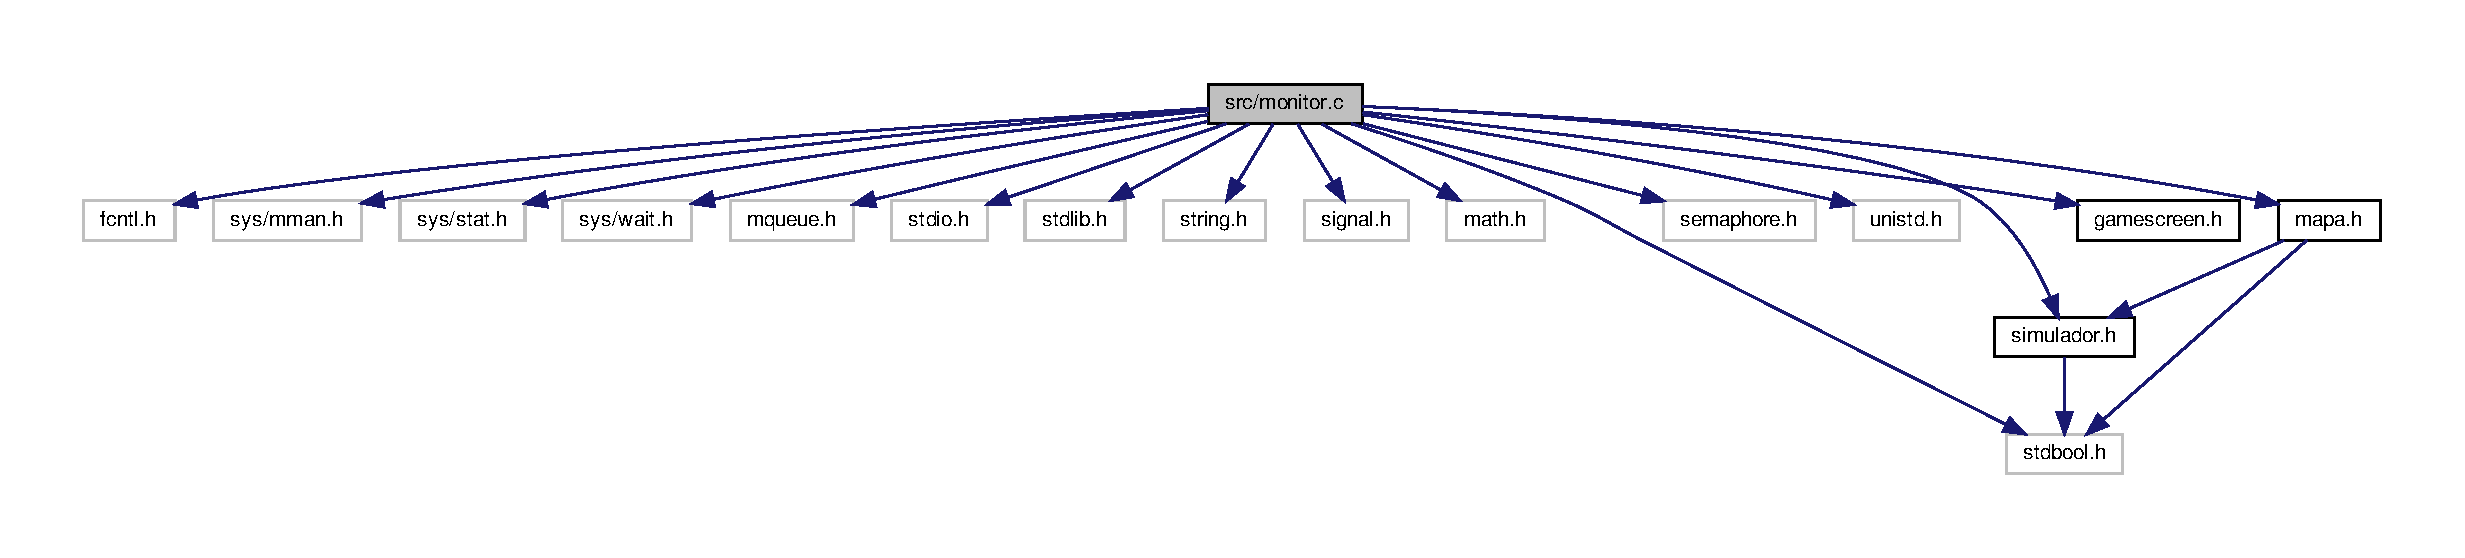
\includegraphics[width=350pt]{monitor_8c__incl}
\end{center}
\end{figure}
\subsection*{Macros}
\begin{DoxyCompactItemize}
\item 
\#define \hyperlink{monitor_8c_a1d1734c6fa929d193aec55de06e7696b}{S\+E\+M\+\_\+\+M\+O\+N\+I\+T\+OR}~\char`\"{}/sem\+\_\+monitor\char`\"{}
\item 
\#define \hyperlink{monitor_8c_a7f83737b56b4e79d52e6869a1ad19d50}{M\+U\+T\+E\+X\+\_\+\+M\+A\+PA}~\char`\"{}/sem\+\_\+mutex\+\_\+mapa\char`\"{}
\item 
\#define \hyperlink{monitor_8c_af3e24bb2a924e231bc8e631939537488}{S\+H\+M\+\_\+\+M\+A\+PA}~\char`\"{}/shm\+\_\+estado\char`\"{}
\end{DoxyCompactItemize}
\subsection*{Functions}
\begin{DoxyCompactItemize}
\item 
void \hyperlink{monitor_8c_a19b6b23fdb523f12cdc3a096dcd92d25}{mapa\+\_\+print} (\hyperlink{structtipo__mapa}{tipo\+\_\+mapa} $\ast$\hyperlink{simulador_8c_a3f88248411450095465da3e38eb812c2}{mapa})
\begin{DoxyCompactList}\small\item\em \+: Funcion que imprime por pantalla todos los simbolos de las casillas del mapa recibido como parametro. \end{DoxyCompactList}\item 
int \hyperlink{monitor_8c_ae66f6b31b5ad750f1fe042a706a4e3d4}{main} ()
\end{DoxyCompactItemize}


\subsection{Detailed Description}
Programa que muestra el estado de la simulacion en la terminal de forma mas visual. Debe ser ejecutado desde un terminal diferente al del proceso simulador, y finalizado a mano con Ctrl+C. 

\begin{DoxyAuthor}{Author}
Alba Ramos\+: \href{mailto:alba.ramosp@estudiante.uam.es}{\tt alba.\+ramosp@estudiante.\+uam.\+es}; Grupo 2213 

Andrea Salcedo\+: \href{mailto:andrea.salcedo@estudiante.uam.es}{\tt andrea.\+salcedo@estudiante.\+uam.\+es}; Grupo 2213 
\end{DoxyAuthor}
\begin{DoxyDate}{Date}
11-\/04-\/2019 
\end{DoxyDate}


\subsection{Macro Definition Documentation}
\mbox{\Hypertarget{monitor_8c_a7f83737b56b4e79d52e6869a1ad19d50}\label{monitor_8c_a7f83737b56b4e79d52e6869a1ad19d50}} 
\index{monitor.\+c@{monitor.\+c}!M\+U\+T\+E\+X\+\_\+\+M\+A\+PA@{M\+U\+T\+E\+X\+\_\+\+M\+A\+PA}}
\index{M\+U\+T\+E\+X\+\_\+\+M\+A\+PA@{M\+U\+T\+E\+X\+\_\+\+M\+A\+PA}!monitor.\+c@{monitor.\+c}}
\subsubsection{\texorpdfstring{M\+U\+T\+E\+X\+\_\+\+M\+A\+PA}{MUTEX\_MAPA}}
{\footnotesize\ttfamily \#define M\+U\+T\+E\+X\+\_\+\+M\+A\+PA~\char`\"{}/sem\+\_\+mutex\+\_\+mapa\char`\"{}}

\mbox{\Hypertarget{monitor_8c_a1d1734c6fa929d193aec55de06e7696b}\label{monitor_8c_a1d1734c6fa929d193aec55de06e7696b}} 
\index{monitor.\+c@{monitor.\+c}!S\+E\+M\+\_\+\+M\+O\+N\+I\+T\+OR@{S\+E\+M\+\_\+\+M\+O\+N\+I\+T\+OR}}
\index{S\+E\+M\+\_\+\+M\+O\+N\+I\+T\+OR@{S\+E\+M\+\_\+\+M\+O\+N\+I\+T\+OR}!monitor.\+c@{monitor.\+c}}
\subsubsection{\texorpdfstring{S\+E\+M\+\_\+\+M\+O\+N\+I\+T\+OR}{SEM\_MONITOR}}
{\footnotesize\ttfamily \#define S\+E\+M\+\_\+\+M\+O\+N\+I\+T\+OR~\char`\"{}/sem\+\_\+monitor\char`\"{}}

\mbox{\Hypertarget{monitor_8c_af3e24bb2a924e231bc8e631939537488}\label{monitor_8c_af3e24bb2a924e231bc8e631939537488}} 
\index{monitor.\+c@{monitor.\+c}!S\+H\+M\+\_\+\+M\+A\+PA@{S\+H\+M\+\_\+\+M\+A\+PA}}
\index{S\+H\+M\+\_\+\+M\+A\+PA@{S\+H\+M\+\_\+\+M\+A\+PA}!monitor.\+c@{monitor.\+c}}
\subsubsection{\texorpdfstring{S\+H\+M\+\_\+\+M\+A\+PA}{SHM\_MAPA}}
{\footnotesize\ttfamily \#define S\+H\+M\+\_\+\+M\+A\+PA~\char`\"{}/shm\+\_\+estado\char`\"{}}



\subsection{Function Documentation}
\mbox{\Hypertarget{monitor_8c_ae66f6b31b5ad750f1fe042a706a4e3d4}\label{monitor_8c_ae66f6b31b5ad750f1fe042a706a4e3d4}} 
\index{monitor.\+c@{monitor.\+c}!main@{main}}
\index{main@{main}!monitor.\+c@{monitor.\+c}}
\subsubsection{\texorpdfstring{main()}{main()}}
{\footnotesize\ttfamily int main (\begin{DoxyParamCaption}{ }\end{DoxyParamCaption})}

\mbox{\Hypertarget{monitor_8c_a19b6b23fdb523f12cdc3a096dcd92d25}\label{monitor_8c_a19b6b23fdb523f12cdc3a096dcd92d25}} 
\index{monitor.\+c@{monitor.\+c}!mapa\+\_\+print@{mapa\+\_\+print}}
\index{mapa\+\_\+print@{mapa\+\_\+print}!monitor.\+c@{monitor.\+c}}
\subsubsection{\texorpdfstring{mapa\+\_\+print()}{mapa\_print()}}
{\footnotesize\ttfamily void mapa\+\_\+print (\begin{DoxyParamCaption}\item[{\hyperlink{structtipo__mapa}{tipo\+\_\+mapa} $\ast$}]{mapa }\end{DoxyParamCaption})}



\+: Funcion que imprime por pantalla todos los simbolos de las casillas del mapa recibido como parametro. 


\begin{DoxyParams}{Parameters}
{\em } & \\
\hline
\end{DoxyParams}

\hypertarget{nave_8c}{}\section{src/nave.c File Reference}
\label{nave_8c}\index{src/nave.\+c@{src/nave.\+c}}


Programa que se encarga de ejecutar el codigo de una nave, el cual recibe una accion enviada por su proceso jefe para posteriormente, enviárselo al simulador para que ejecute las acciones necesarias una vez recibida la información por la Cola de Mensajes.  


{\ttfamily \#include $<$fcntl.\+h$>$}\newline
{\ttfamily \#include $<$sys/mman.\+h$>$}\newline
{\ttfamily \#include $<$sys/stat.\+h$>$}\newline
{\ttfamily \#include $<$sys/wait.\+h$>$}\newline
{\ttfamily \#include $<$mqueue.\+h$>$}\newline
{\ttfamily \#include $<$stdio.\+h$>$}\newline
{\ttfamily \#include $<$stdlib.\+h$>$}\newline
{\ttfamily \#include $<$string.\+h$>$}\newline
{\ttfamily \#include $<$signal.\+h$>$}\newline
{\ttfamily \#include $<$semaphore.\+h$>$}\newline
{\ttfamily \#include $<$math.\+h$>$}\newline
{\ttfamily \#include $<$stdbool.\+h$>$}\newline
{\ttfamily \#include $<$unistd.\+h$>$}\newline
{\ttfamily \#include $<$mapa.\+h$>$}\newline
{\ttfamily \#include $<$time.\+h$>$}\newline
{\ttfamily \#include $<$simulador.\+h$>$}\newline
Include dependency graph for nave.\+c\+:
\nopagebreak
\begin{figure}[H]
\begin{center}
\leavevmode
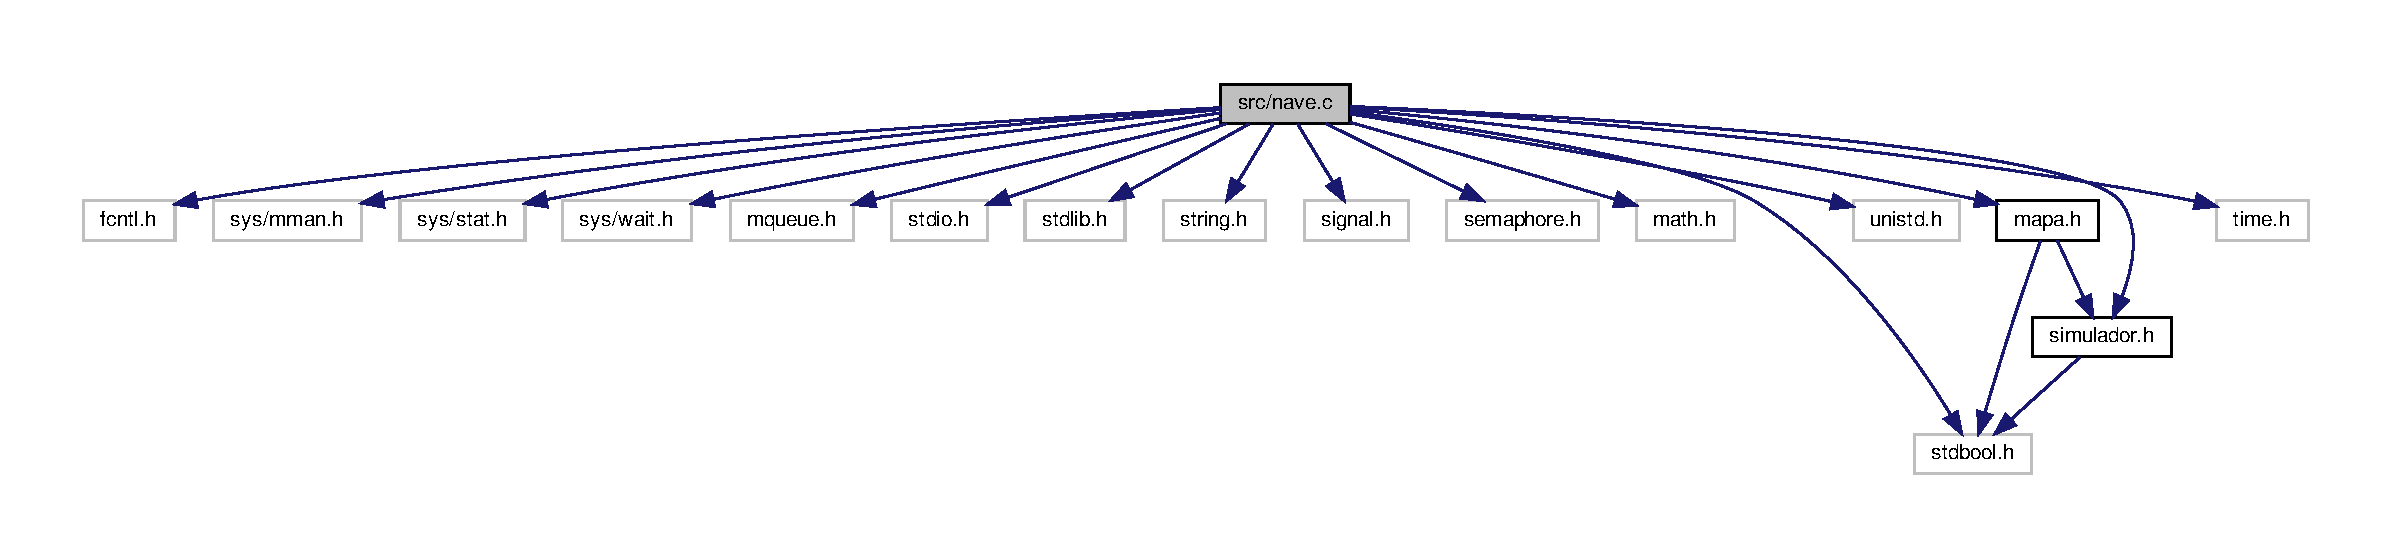
\includegraphics[width=350pt]{nave_8c__incl}
\end{center}
\end{figure}
\subsection*{Macros}
\begin{DoxyCompactItemize}
\item 
\#define \hyperlink{nave_8c_a24f3611c6828c8df80cb2b61dd3f1df4}{M\+Q\+\_\+\+N\+A\+ME}~\char`\"{}/mq\+\_\+nave\+Simulador\char`\"{}
\item 
\#define \hyperlink{nave_8c_a7e904a08f91ace8279e61f3ddd004722}{M\+U\+T\+E\+X\+\_\+\+C\+O\+N\+T\+\_\+C}~\char`\"{}/sem\+\_\+mutex\+\_\+contC\char`\"{}
\item 
\#define \hyperlink{nave_8c_af3e24bb2a924e231bc8e631939537488}{S\+H\+M\+\_\+\+M\+A\+PA}~\char`\"{}/shm\+\_\+estado\char`\"{}
\item 
\#define \hyperlink{nave_8c_a7f83737b56b4e79d52e6869a1ad19d50}{M\+U\+T\+E\+X\+\_\+\+M\+A\+PA}~\char`\"{}/sem\+\_\+mutex\+\_\+mapa\char`\"{}
\item 
\#define \hyperlink{nave_8c_ad8e2b34b5877c257f4d561ceadc9e1c1}{S\+H\+M\+\_\+\+T\+UB}~\char`\"{}/shm\+\_\+tuberias\char`\"{}
\end{DoxyCompactItemize}
\subsection*{Functions}
\begin{DoxyCompactItemize}
\item 
void \hyperlink{nave_8c_a493ad48174879c61a0ed41fdffd829fa}{liberar} ()
\begin{DoxyCompactList}\small\item\em Funcion que se encarga de cerrar todos los recursos de la simulacion. \end{DoxyCompactList}\item 
void \hyperlink{nave_8c_a6f273161e1b40433f3aeab3fdb4613eb}{manejador\+S\+I\+G\+T\+E\+RM} ()
\begin{DoxyCompactList}\small\item\em Funcion que se encarga de manejar la señal S\+I\+G\+T\+E\+RM, enviada por el proceso simulador cuando ha habido un equipo ganador. \end{DoxyCompactList}\item 
int \hyperlink{nave_8c_abf9e6b7e6f15df4b525a2e7705ba3089}{main} (int argc, char const $\ast$argv\mbox{[}$\,$\mbox{]})
\begin{DoxyCompactList}\small\item\em Funcion principal del proceso nave, se encargara de ejecutar todas las acciones una vez recibida la accion por la tuberia. \end{DoxyCompactList}\end{DoxyCompactItemize}
\subsection*{Variables}
\begin{DoxyCompactItemize}
\item 
mqd\+\_\+t \hyperlink{nave_8c_a291a70b5a1b4939b410947fbe1f3a4a7}{cola\+Simulador}
\item 
\hyperlink{structMensaje}{Mensaje} \hyperlink{nave_8c_a2eda5cbc72880acfba91bd43e52f89cd}{msg}
\item 
\hyperlink{structTuberia}{Tuberia} $\ast$ \hyperlink{nave_8c_a677056758f5c7c430c4b6cb2543d138b}{tuberia}
\item 
int \hyperlink{nave_8c_ab2944d7491ac51f8acc448d0a23f1da8}{memoria\+Tuberia}
\item 
sem\+\_\+t $\ast$ \hyperlink{nave_8c_a41552ad512e099bbd1441ad05cc4a106}{mutex\+Mapa} = N\+U\+LL
\item 
int \hyperlink{nave_8c_afc2453dbc73f5ea89d86807d62f4931a}{memoria\+Estado}
\item 
\hyperlink{structtipo__mapa}{tipo\+\_\+mapa} $\ast$ \hyperlink{nave_8c_a3f88248411450095465da3e38eb812c2}{mapa}
\item 
int \hyperlink{nave_8c_aa5e6716194f228a7cc36e89f613a30d0}{equipo}
\item 
int \hyperlink{nave_8c_ad8ebb14676f9e6705b02b689d70592aa}{n\+Nave}
\item 
sem\+\_\+t $\ast$ \hyperlink{nave_8c_abf90b199b02e2b4ed8c05d34c06d9e7c}{mutex\+ContC} = N\+U\+LL
\item 
struct sigaction \hyperlink{nave_8c_a2c79c9e74cc5711454ff7456a4c56214}{act2}
\end{DoxyCompactItemize}


\subsection{Detailed Description}
Programa que se encarga de ejecutar el codigo de una nave, el cual recibe una accion enviada por su proceso jefe para posteriormente, enviárselo al simulador para que ejecute las acciones necesarias una vez recibida la información por la Cola de Mensajes. 

\begin{DoxyAuthor}{Author}
Alba Ramos\+: \href{mailto:alba.ramosp@estudiante.uam.es}{\tt alba.\+ramosp@estudiante.\+uam.\+es}; Grupo 2213 

Andrea Salcedo\+: \href{mailto:andrea.salcedo@estudiante.uam.es}{\tt andrea.\+salcedo@estudiante.\+uam.\+es}; Grupo 2213 
\end{DoxyAuthor}
\begin{DoxyDate}{Date}
11-\/04-\/2019 
\end{DoxyDate}


\subsection{Macro Definition Documentation}
\mbox{\Hypertarget{nave_8c_a24f3611c6828c8df80cb2b61dd3f1df4}\label{nave_8c_a24f3611c6828c8df80cb2b61dd3f1df4}} 
\index{nave.\+c@{nave.\+c}!M\+Q\+\_\+\+N\+A\+ME@{M\+Q\+\_\+\+N\+A\+ME}}
\index{M\+Q\+\_\+\+N\+A\+ME@{M\+Q\+\_\+\+N\+A\+ME}!nave.\+c@{nave.\+c}}
\subsubsection{\texorpdfstring{M\+Q\+\_\+\+N\+A\+ME}{MQ\_NAME}}
{\footnotesize\ttfamily \#define M\+Q\+\_\+\+N\+A\+ME~\char`\"{}/mq\+\_\+nave\+Simulador\char`\"{}}

\mbox{\Hypertarget{nave_8c_a7e904a08f91ace8279e61f3ddd004722}\label{nave_8c_a7e904a08f91ace8279e61f3ddd004722}} 
\index{nave.\+c@{nave.\+c}!M\+U\+T\+E\+X\+\_\+\+C\+O\+N\+T\+\_\+C@{M\+U\+T\+E\+X\+\_\+\+C\+O\+N\+T\+\_\+C}}
\index{M\+U\+T\+E\+X\+\_\+\+C\+O\+N\+T\+\_\+C@{M\+U\+T\+E\+X\+\_\+\+C\+O\+N\+T\+\_\+C}!nave.\+c@{nave.\+c}}
\subsubsection{\texorpdfstring{M\+U\+T\+E\+X\+\_\+\+C\+O\+N\+T\+\_\+C}{MUTEX\_CONT\_C}}
{\footnotesize\ttfamily \#define M\+U\+T\+E\+X\+\_\+\+C\+O\+N\+T\+\_\+C~\char`\"{}/sem\+\_\+mutex\+\_\+contC\char`\"{}}

\mbox{\Hypertarget{nave_8c_a7f83737b56b4e79d52e6869a1ad19d50}\label{nave_8c_a7f83737b56b4e79d52e6869a1ad19d50}} 
\index{nave.\+c@{nave.\+c}!M\+U\+T\+E\+X\+\_\+\+M\+A\+PA@{M\+U\+T\+E\+X\+\_\+\+M\+A\+PA}}
\index{M\+U\+T\+E\+X\+\_\+\+M\+A\+PA@{M\+U\+T\+E\+X\+\_\+\+M\+A\+PA}!nave.\+c@{nave.\+c}}
\subsubsection{\texorpdfstring{M\+U\+T\+E\+X\+\_\+\+M\+A\+PA}{MUTEX\_MAPA}}
{\footnotesize\ttfamily \#define M\+U\+T\+E\+X\+\_\+\+M\+A\+PA~\char`\"{}/sem\+\_\+mutex\+\_\+mapa\char`\"{}}

\mbox{\Hypertarget{nave_8c_af3e24bb2a924e231bc8e631939537488}\label{nave_8c_af3e24bb2a924e231bc8e631939537488}} 
\index{nave.\+c@{nave.\+c}!S\+H\+M\+\_\+\+M\+A\+PA@{S\+H\+M\+\_\+\+M\+A\+PA}}
\index{S\+H\+M\+\_\+\+M\+A\+PA@{S\+H\+M\+\_\+\+M\+A\+PA}!nave.\+c@{nave.\+c}}
\subsubsection{\texorpdfstring{S\+H\+M\+\_\+\+M\+A\+PA}{SHM\_MAPA}}
{\footnotesize\ttfamily \#define S\+H\+M\+\_\+\+M\+A\+PA~\char`\"{}/shm\+\_\+estado\char`\"{}}

\mbox{\Hypertarget{nave_8c_ad8e2b34b5877c257f4d561ceadc9e1c1}\label{nave_8c_ad8e2b34b5877c257f4d561ceadc9e1c1}} 
\index{nave.\+c@{nave.\+c}!S\+H\+M\+\_\+\+T\+UB@{S\+H\+M\+\_\+\+T\+UB}}
\index{S\+H\+M\+\_\+\+T\+UB@{S\+H\+M\+\_\+\+T\+UB}!nave.\+c@{nave.\+c}}
\subsubsection{\texorpdfstring{S\+H\+M\+\_\+\+T\+UB}{SHM\_TUB}}
{\footnotesize\ttfamily \#define S\+H\+M\+\_\+\+T\+UB~\char`\"{}/shm\+\_\+tuberias\char`\"{}}



\subsection{Function Documentation}
\mbox{\Hypertarget{nave_8c_a493ad48174879c61a0ed41fdffd829fa}\label{nave_8c_a493ad48174879c61a0ed41fdffd829fa}} 
\index{nave.\+c@{nave.\+c}!liberar@{liberar}}
\index{liberar@{liberar}!nave.\+c@{nave.\+c}}
\subsubsection{\texorpdfstring{liberar()}{liberar()}}
{\footnotesize\ttfamily void liberar (\begin{DoxyParamCaption}{ }\end{DoxyParamCaption})}



Funcion que se encarga de cerrar todos los recursos de la simulacion. 

\begin{DoxyReturn}{Returns}
void libera los recursos y finaliza 
\end{DoxyReturn}
\mbox{\Hypertarget{nave_8c_abf9e6b7e6f15df4b525a2e7705ba3089}\label{nave_8c_abf9e6b7e6f15df4b525a2e7705ba3089}} 
\index{nave.\+c@{nave.\+c}!main@{main}}
\index{main@{main}!nave.\+c@{nave.\+c}}
\subsubsection{\texorpdfstring{main()}{main()}}
{\footnotesize\ttfamily int main (\begin{DoxyParamCaption}\item[{int}]{argc,  }\item[{char const $\ast$}]{argv\mbox{[}$\,$\mbox{]} }\end{DoxyParamCaption})}



Funcion principal del proceso nave, se encargara de ejecutar todas las acciones una vez recibida la accion por la tuberia. 


\begin{DoxyParams}{Parameters}
{\em argc} & int, argv\+: char const \\
\hline
\end{DoxyParams}
\begin{DoxyReturn}{Returns}
devuelve E\+X\+I\+T\+\_\+\+S\+U\+C\+C\+E\+SS si todo ha ido correctamente 
\end{DoxyReturn}
Abrimos los recursos creados en el simulador para poder usarlos en la nave

Inicializamos el contador\+Cola para contabilizar el numero de naves que van a enviar información al simulador

Bucle en el que vamos a procesar las acciones recibidas \mbox{\Hypertarget{nave_8c_a6f273161e1b40433f3aeab3fdb4613eb}\label{nave_8c_a6f273161e1b40433f3aeab3fdb4613eb}} 
\index{nave.\+c@{nave.\+c}!manejador\+S\+I\+G\+T\+E\+RM@{manejador\+S\+I\+G\+T\+E\+RM}}
\index{manejador\+S\+I\+G\+T\+E\+RM@{manejador\+S\+I\+G\+T\+E\+RM}!nave.\+c@{nave.\+c}}
\subsubsection{\texorpdfstring{manejador\+S\+I\+G\+T\+E\+R\+M()}{manejadorSIGTERM()}}
{\footnotesize\ttfamily void manejador\+S\+I\+G\+T\+E\+RM (\begin{DoxyParamCaption}{ }\end{DoxyParamCaption})}



Funcion que se encarga de manejar la señal S\+I\+G\+T\+E\+RM, enviada por el proceso simulador cuando ha habido un equipo ganador. 

\begin{DoxyReturn}{Returns}
void, termina la ejecucion de una nave 
\end{DoxyReturn}


\subsection{Variable Documentation}
\mbox{\Hypertarget{nave_8c_a2c79c9e74cc5711454ff7456a4c56214}\label{nave_8c_a2c79c9e74cc5711454ff7456a4c56214}} 
\index{nave.\+c@{nave.\+c}!act2@{act2}}
\index{act2@{act2}!nave.\+c@{nave.\+c}}
\subsubsection{\texorpdfstring{act2}{act2}}
{\footnotesize\ttfamily struct sigaction act2}

Estructura para la captura de señales, en este caso la de S\+I\+G\+T\+E\+RM \mbox{\Hypertarget{nave_8c_a291a70b5a1b4939b410947fbe1f3a4a7}\label{nave_8c_a291a70b5a1b4939b410947fbe1f3a4a7}} 
\index{nave.\+c@{nave.\+c}!cola\+Simulador@{cola\+Simulador}}
\index{cola\+Simulador@{cola\+Simulador}!nave.\+c@{nave.\+c}}
\subsubsection{\texorpdfstring{cola\+Simulador}{colaSimulador}}
{\footnotesize\ttfamily mqd\+\_\+t cola\+Simulador}

Cola de mensajes, para la comunicacion entre naves-\/simulador \mbox{\Hypertarget{nave_8c_aa5e6716194f228a7cc36e89f613a30d0}\label{nave_8c_aa5e6716194f228a7cc36e89f613a30d0}} 
\index{nave.\+c@{nave.\+c}!equipo@{equipo}}
\index{equipo@{equipo}!nave.\+c@{nave.\+c}}
\subsubsection{\texorpdfstring{equipo}{equipo}}
{\footnotesize\ttfamily int equipo}

Variable global que almacena el numero de equipo de la nave, el cual es dado por argumento \mbox{\Hypertarget{nave_8c_a3f88248411450095465da3e38eb812c2}\label{nave_8c_a3f88248411450095465da3e38eb812c2}} 
\index{nave.\+c@{nave.\+c}!mapa@{mapa}}
\index{mapa@{mapa}!nave.\+c@{nave.\+c}}
\subsubsection{\texorpdfstring{mapa}{mapa}}
{\footnotesize\ttfamily \hyperlink{structtipo__mapa}{tipo\+\_\+mapa}$\ast$ mapa}

\mbox{\Hypertarget{nave_8c_afc2453dbc73f5ea89d86807d62f4931a}\label{nave_8c_afc2453dbc73f5ea89d86807d62f4931a}} 
\index{nave.\+c@{nave.\+c}!memoria\+Estado@{memoria\+Estado}}
\index{memoria\+Estado@{memoria\+Estado}!nave.\+c@{nave.\+c}}
\subsubsection{\texorpdfstring{memoria\+Estado}{memoriaEstado}}
{\footnotesize\ttfamily int memoria\+Estado}

Memoria compartida para el mapa, la usaremos para poder realizar la accion de M\+O\+V\+ER a una posicioón aleatoria \mbox{\Hypertarget{nave_8c_ab2944d7491ac51f8acc448d0a23f1da8}\label{nave_8c_ab2944d7491ac51f8acc448d0a23f1da8}} 
\index{nave.\+c@{nave.\+c}!memoria\+Tuberia@{memoria\+Tuberia}}
\index{memoria\+Tuberia@{memoria\+Tuberia}!nave.\+c@{nave.\+c}}
\subsubsection{\texorpdfstring{memoria\+Tuberia}{memoriaTuberia}}
{\footnotesize\ttfamily int memoria\+Tuberia}

Memoria compartida que almacena los descriptores de fichero de los diferentes pipes tanto de los jefes como de las naves. \mbox{\Hypertarget{nave_8c_a2eda5cbc72880acfba91bd43e52f89cd}\label{nave_8c_a2eda5cbc72880acfba91bd43e52f89cd}} 
\index{nave.\+c@{nave.\+c}!msg@{msg}}
\index{msg@{msg}!nave.\+c@{nave.\+c}}
\subsubsection{\texorpdfstring{msg}{msg}}
{\footnotesize\ttfamily \hyperlink{structMensaje}{Mensaje} msg}

Variable que apunta a la estructura \hyperlink{structMensaje}{Mensaje} del simulador. \mbox{\Hypertarget{nave_8c_abf90b199b02e2b4ed8c05d34c06d9e7c}\label{nave_8c_abf90b199b02e2b4ed8c05d34c06d9e7c}} 
\index{nave.\+c@{nave.\+c}!mutex\+ContC@{mutex\+ContC}}
\index{mutex\+ContC@{mutex\+ContC}!nave.\+c@{nave.\+c}}
\subsubsection{\texorpdfstring{mutex\+ContC}{mutexContC}}
{\footnotesize\ttfamily sem\+\_\+t$\ast$ mutex\+ContC = N\+U\+LL}

Semaforo que se encarga de controlar el uso del contador\+Cola \mbox{\Hypertarget{nave_8c_a41552ad512e099bbd1441ad05cc4a106}\label{nave_8c_a41552ad512e099bbd1441ad05cc4a106}} 
\index{nave.\+c@{nave.\+c}!mutex\+Mapa@{mutex\+Mapa}}
\index{mutex\+Mapa@{mutex\+Mapa}!nave.\+c@{nave.\+c}}
\subsubsection{\texorpdfstring{mutex\+Mapa}{mutexMapa}}
{\footnotesize\ttfamily sem\+\_\+t$\ast$ mutex\+Mapa = N\+U\+LL}

Este semaforo controla la entrada de naves en la memoria compartida del mapa, para que solo puedan consultarlo de uno en uno \mbox{\Hypertarget{nave_8c_ad8ebb14676f9e6705b02b689d70592aa}\label{nave_8c_ad8ebb14676f9e6705b02b689d70592aa}} 
\index{nave.\+c@{nave.\+c}!n\+Nave@{n\+Nave}}
\index{n\+Nave@{n\+Nave}!nave.\+c@{nave.\+c}}
\subsubsection{\texorpdfstring{n\+Nave}{nNave}}
{\footnotesize\ttfamily int n\+Nave}

Variable global que almacena el numero de nave de las naves del equipo, el cual es dado por argumento \mbox{\Hypertarget{nave_8c_a677056758f5c7c430c4b6cb2543d138b}\label{nave_8c_a677056758f5c7c430c4b6cb2543d138b}} 
\index{nave.\+c@{nave.\+c}!tuberia@{tuberia}}
\index{tuberia@{tuberia}!nave.\+c@{nave.\+c}}
\subsubsection{\texorpdfstring{tuberia}{tuberia}}
{\footnotesize\ttfamily \hyperlink{structTuberia}{Tuberia}$\ast$ tuberia}


\hypertarget{simulador_8c}{}\section{src/simulador.c File Reference}
\label{simulador_8c}\index{src/simulador.\+c@{src/simulador.\+c}}


Programa que gestiona el funcionamiento principal del proyecto. Se encarga de gestionar los turnos, detectar el fin de la simulacion y procesar las acciones recibidas de las naves.  


{\ttfamily \#include $<$fcntl.\+h$>$}\newline
{\ttfamily \#include $<$errno.\+h$>$}\newline
{\ttfamily \#include $<$sys/mman.\+h$>$}\newline
{\ttfamily \#include $<$sys/stat.\+h$>$}\newline
{\ttfamily \#include $<$sys/wait.\+h$>$}\newline
{\ttfamily \#include $<$mqueue.\+h$>$}\newline
{\ttfamily \#include $<$stdio.\+h$>$}\newline
{\ttfamily \#include $<$stdlib.\+h$>$}\newline
{\ttfamily \#include $<$string.\+h$>$}\newline
{\ttfamily \#include $<$signal.\+h$>$}\newline
{\ttfamily \#include $<$math.\+h$>$}\newline
{\ttfamily \#include $<$stdbool.\+h$>$}\newline
{\ttfamily \#include $<$semaphore.\+h$>$}\newline
{\ttfamily \#include $<$unistd.\+h$>$}\newline
{\ttfamily \#include $<$time.\+h$>$}\newline
{\ttfamily \#include $<$mapa.\+h$>$}\newline
Include dependency graph for simulador.\+c\+:
\nopagebreak
\begin{figure}[H]
\begin{center}
\leavevmode
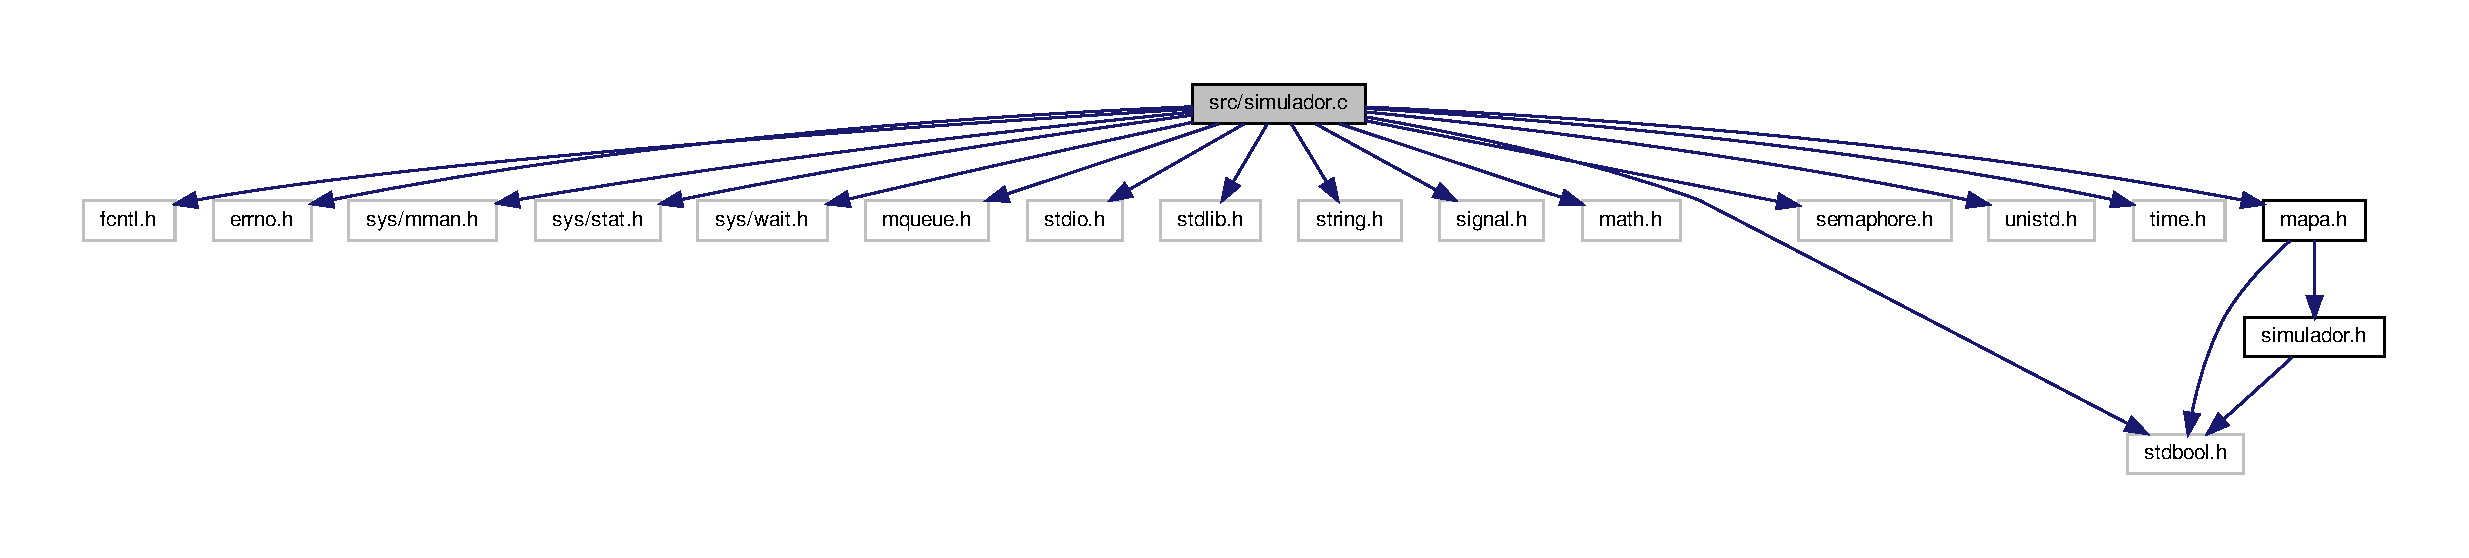
\includegraphics[width=350pt]{simulador_8c__incl}
\end{center}
\end{figure}
\subsection*{Macros}
\begin{DoxyCompactItemize}
\item 
\#define \hyperlink{simulador_8c_aaf0952059602752258dccaa015d7b54a}{N\+UM}~100
\item 
\#define \hyperlink{simulador_8c_a24f3611c6828c8df80cb2b61dd3f1df4}{M\+Q\+\_\+\+N\+A\+ME}~\char`\"{}/mq\+\_\+nave\+Simulador\char`\"{}
\item 
\#define \hyperlink{simulador_8c_af3e24bb2a924e231bc8e631939537488}{S\+H\+M\+\_\+\+M\+A\+PA}~\char`\"{}/shm\+\_\+estado\char`\"{}
\item 
\#define \hyperlink{simulador_8c_ad8e2b34b5877c257f4d561ceadc9e1c1}{S\+H\+M\+\_\+\+T\+UB}~\char`\"{}/shm\+\_\+tuberias\char`\"{}
\item 
\#define \hyperlink{simulador_8c_a05ed14902c0444174e5a14678e806b95}{S\+H\+M\+\_\+\+C\+O\+N\+TC}~\char`\"{}/shm\+\_\+cont\+Cola\char`\"{}
\item 
\#define \hyperlink{simulador_8c_a7e904a08f91ace8279e61f3ddd004722}{M\+U\+T\+E\+X\+\_\+\+C\+O\+N\+T\+\_\+C}~\char`\"{}/sem\+\_\+mutex\+\_\+contC\char`\"{}
\item 
\#define \hyperlink{simulador_8c_a7f83737b56b4e79d52e6869a1ad19d50}{M\+U\+T\+E\+X\+\_\+\+M\+A\+PA}~\char`\"{}/sem\+\_\+mutex\+\_\+mapa\char`\"{}
\item 
\#define \hyperlink{simulador_8c_a486c681bc9fcbd82d87b80a479e6f72d}{S\+E\+M\+\_\+\+J\+E\+F\+ES}~\char`\"{}/sem\+\_\+jefes\char`\"{}
\item 
\#define \hyperlink{simulador_8c_a1d1734c6fa929d193aec55de06e7696b}{S\+E\+M\+\_\+\+M\+O\+N\+I\+T\+OR}~\char`\"{}/sem\+\_\+monitor\char`\"{}
\end{DoxyCompactItemize}
\subsection*{Functions}
\begin{DoxyCompactItemize}
\item 
void \hyperlink{simulador_8c_a493ad48174879c61a0ed41fdffd829fa}{liberar} ()
\begin{DoxyCompactList}\small\item\em Funcion para liberar los recursos. \end{DoxyCompactList}\item 
void \hyperlink{simulador_8c_a8599933c104a4298ae42fe5a69e55b9f}{manejador\+Final} ()
\begin{DoxyCompactList}\small\item\em Manejador de la senyal de Ctrl+C y de S\+I\+G\+T\+E\+RM. En el se liberan los recursos y se avisa del final de la simulacion a los jefes. \end{DoxyCompactList}\item 
void \hyperlink{simulador_8c_a2ef1cf21f76a62fa2417391f5a54a405}{manejador\+Turno} ()
\begin{DoxyCompactList}\small\item\em Manejador de la senyal de alarma para turnos, que cambia el valor del flag para indicar que se debe mandar una nueva alarma. \end{DoxyCompactList}\item 
int \hyperlink{simulador_8c_abf9e6b7e6f15df4b525a2e7705ba3089}{main} (int argc, char const $\ast$argv\mbox{[}$\,$\mbox{]})
\end{DoxyCompactItemize}
\subsection*{Variables}
\begin{DoxyCompactItemize}
\item 
int \hyperlink{simulador_8c_afc2453dbc73f5ea89d86807d62f4931a}{memoria\+Estado}
\item 
\hyperlink{structtipo__mapa}{tipo\+\_\+mapa} $\ast$ \hyperlink{simulador_8c_a3f88248411450095465da3e38eb812c2}{mapa}
\item 
\hyperlink{structtipo__nave}{tipo\+\_\+nave} \hyperlink{simulador_8c_a07b840f96eed6f1047e59f13647a2b46}{naves} \mbox{[}\hyperlink{simulador_8h_ab306668933fb4316ac0f5ef291d13dff}{N\+\_\+\+E\+Q\+U\+I\+P\+OS}\mbox{]}\mbox{[}\hyperlink{simulador_8h_aa1f2aba814c6d46772f9694849eeaa7a}{N\+\_\+\+N\+A\+V\+ES}\mbox{]}
\item 
sem\+\_\+t $\ast$ \hyperlink{simulador_8c_abf90b199b02e2b4ed8c05d34c06d9e7c}{mutex\+ContC} = N\+U\+LL
\item 
sem\+\_\+t $\ast$ \hyperlink{simulador_8c_a41552ad512e099bbd1441ad05cc4a106}{mutex\+Mapa} = N\+U\+LL
\item 
sem\+\_\+t $\ast$ \hyperlink{simulador_8c_addb0adf902152934d52498fad43752e4}{sem\+\_\+jefes} = N\+U\+LL
\item 
sem\+\_\+t $\ast$ \hyperlink{simulador_8c_a96c1d91b1760b38aeb594b8de3617148}{sem\+\_\+monitor} = N\+U\+LL
\item 
\hyperlink{structTuberia}{Tuberia} $\ast$ \hyperlink{simulador_8c_a3d310fa17a6f70f6981d7056d44ea84a}{tuberias}
\item 
int \hyperlink{simulador_8c_a192ceef35c192084a53e01a0e52487ae}{memoria\+Tuberias}
\item 
mqd\+\_\+t \hyperlink{simulador_8c_a291a70b5a1b4939b410947fbe1f3a4a7}{cola\+Simulador}
\item 
struct mq\+\_\+attr \hyperlink{simulador_8c_ab4509483f1141585c52e3ecf14353934}{attributes}
\item 
struct sigaction \hyperlink{simulador_8c_ae99b99d988ca0b59c3ac838c12751cfe}{act}
\item 
struct sigaction \hyperlink{simulador_8c_a2c79c9e74cc5711454ff7456a4c56214}{act2}
\item 
int \hyperlink{simulador_8c_adf916204820072417ed73a32de1cefcf}{flag} = 0
\item 
\hyperlink{structMensaje}{Mensaje} \hyperlink{simulador_8c_a2eda5cbc72880acfba91bd43e52f89cd}{msg}
\item 
\hyperlink{structOrden}{Orden} \hyperlink{simulador_8c_a8bafa219354a73993a9146dd99a478b9}{orden}
\end{DoxyCompactItemize}


\subsection{Detailed Description}
Programa que gestiona el funcionamiento principal del proyecto. Se encarga de gestionar los turnos, detectar el fin de la simulacion y procesar las acciones recibidas de las naves. 

\begin{DoxyAuthor}{Author}
Alba Ramos\+: \href{mailto:alba.ramosp@estudiante.uam.es}{\tt alba.\+ramosp@estudiante.\+uam.\+es}; Grupo 2213 

Andrea Salcedo\+: \href{mailto:andrea.salcedo@estudiante.uam.es}{\tt andrea.\+salcedo@estudiante.\+uam.\+es}; Grupo 2213 
\end{DoxyAuthor}
\begin{DoxyDate}{Date}
11-\/04-\/2019 
\end{DoxyDate}


\subsection{Macro Definition Documentation}
\mbox{\Hypertarget{simulador_8c_a24f3611c6828c8df80cb2b61dd3f1df4}\label{simulador_8c_a24f3611c6828c8df80cb2b61dd3f1df4}} 
\index{simulador.\+c@{simulador.\+c}!M\+Q\+\_\+\+N\+A\+ME@{M\+Q\+\_\+\+N\+A\+ME}}
\index{M\+Q\+\_\+\+N\+A\+ME@{M\+Q\+\_\+\+N\+A\+ME}!simulador.\+c@{simulador.\+c}}
\subsubsection{\texorpdfstring{M\+Q\+\_\+\+N\+A\+ME}{MQ\_NAME}}
{\footnotesize\ttfamily \#define M\+Q\+\_\+\+N\+A\+ME~\char`\"{}/mq\+\_\+nave\+Simulador\char`\"{}}

\mbox{\Hypertarget{simulador_8c_a7e904a08f91ace8279e61f3ddd004722}\label{simulador_8c_a7e904a08f91ace8279e61f3ddd004722}} 
\index{simulador.\+c@{simulador.\+c}!M\+U\+T\+E\+X\+\_\+\+C\+O\+N\+T\+\_\+C@{M\+U\+T\+E\+X\+\_\+\+C\+O\+N\+T\+\_\+C}}
\index{M\+U\+T\+E\+X\+\_\+\+C\+O\+N\+T\+\_\+C@{M\+U\+T\+E\+X\+\_\+\+C\+O\+N\+T\+\_\+C}!simulador.\+c@{simulador.\+c}}
\subsubsection{\texorpdfstring{M\+U\+T\+E\+X\+\_\+\+C\+O\+N\+T\+\_\+C}{MUTEX\_CONT\_C}}
{\footnotesize\ttfamily \#define M\+U\+T\+E\+X\+\_\+\+C\+O\+N\+T\+\_\+C~\char`\"{}/sem\+\_\+mutex\+\_\+contC\char`\"{}}

\mbox{\Hypertarget{simulador_8c_a7f83737b56b4e79d52e6869a1ad19d50}\label{simulador_8c_a7f83737b56b4e79d52e6869a1ad19d50}} 
\index{simulador.\+c@{simulador.\+c}!M\+U\+T\+E\+X\+\_\+\+M\+A\+PA@{M\+U\+T\+E\+X\+\_\+\+M\+A\+PA}}
\index{M\+U\+T\+E\+X\+\_\+\+M\+A\+PA@{M\+U\+T\+E\+X\+\_\+\+M\+A\+PA}!simulador.\+c@{simulador.\+c}}
\subsubsection{\texorpdfstring{M\+U\+T\+E\+X\+\_\+\+M\+A\+PA}{MUTEX\_MAPA}}
{\footnotesize\ttfamily \#define M\+U\+T\+E\+X\+\_\+\+M\+A\+PA~\char`\"{}/sem\+\_\+mutex\+\_\+mapa\char`\"{}}

\mbox{\Hypertarget{simulador_8c_aaf0952059602752258dccaa015d7b54a}\label{simulador_8c_aaf0952059602752258dccaa015d7b54a}} 
\index{simulador.\+c@{simulador.\+c}!N\+UM@{N\+UM}}
\index{N\+UM@{N\+UM}!simulador.\+c@{simulador.\+c}}
\subsubsection{\texorpdfstring{N\+UM}{NUM}}
{\footnotesize\ttfamily \#define N\+UM~100}

\mbox{\Hypertarget{simulador_8c_a486c681bc9fcbd82d87b80a479e6f72d}\label{simulador_8c_a486c681bc9fcbd82d87b80a479e6f72d}} 
\index{simulador.\+c@{simulador.\+c}!S\+E\+M\+\_\+\+J\+E\+F\+ES@{S\+E\+M\+\_\+\+J\+E\+F\+ES}}
\index{S\+E\+M\+\_\+\+J\+E\+F\+ES@{S\+E\+M\+\_\+\+J\+E\+F\+ES}!simulador.\+c@{simulador.\+c}}
\subsubsection{\texorpdfstring{S\+E\+M\+\_\+\+J\+E\+F\+ES}{SEM\_JEFES}}
{\footnotesize\ttfamily \#define S\+E\+M\+\_\+\+J\+E\+F\+ES~\char`\"{}/sem\+\_\+jefes\char`\"{}}

\mbox{\Hypertarget{simulador_8c_a1d1734c6fa929d193aec55de06e7696b}\label{simulador_8c_a1d1734c6fa929d193aec55de06e7696b}} 
\index{simulador.\+c@{simulador.\+c}!S\+E\+M\+\_\+\+M\+O\+N\+I\+T\+OR@{S\+E\+M\+\_\+\+M\+O\+N\+I\+T\+OR}}
\index{S\+E\+M\+\_\+\+M\+O\+N\+I\+T\+OR@{S\+E\+M\+\_\+\+M\+O\+N\+I\+T\+OR}!simulador.\+c@{simulador.\+c}}
\subsubsection{\texorpdfstring{S\+E\+M\+\_\+\+M\+O\+N\+I\+T\+OR}{SEM\_MONITOR}}
{\footnotesize\ttfamily \#define S\+E\+M\+\_\+\+M\+O\+N\+I\+T\+OR~\char`\"{}/sem\+\_\+monitor\char`\"{}}

\mbox{\Hypertarget{simulador_8c_a05ed14902c0444174e5a14678e806b95}\label{simulador_8c_a05ed14902c0444174e5a14678e806b95}} 
\index{simulador.\+c@{simulador.\+c}!S\+H\+M\+\_\+\+C\+O\+N\+TC@{S\+H\+M\+\_\+\+C\+O\+N\+TC}}
\index{S\+H\+M\+\_\+\+C\+O\+N\+TC@{S\+H\+M\+\_\+\+C\+O\+N\+TC}!simulador.\+c@{simulador.\+c}}
\subsubsection{\texorpdfstring{S\+H\+M\+\_\+\+C\+O\+N\+TC}{SHM\_CONTC}}
{\footnotesize\ttfamily \#define S\+H\+M\+\_\+\+C\+O\+N\+TC~\char`\"{}/shm\+\_\+cont\+Cola\char`\"{}}

\mbox{\Hypertarget{simulador_8c_af3e24bb2a924e231bc8e631939537488}\label{simulador_8c_af3e24bb2a924e231bc8e631939537488}} 
\index{simulador.\+c@{simulador.\+c}!S\+H\+M\+\_\+\+M\+A\+PA@{S\+H\+M\+\_\+\+M\+A\+PA}}
\index{S\+H\+M\+\_\+\+M\+A\+PA@{S\+H\+M\+\_\+\+M\+A\+PA}!simulador.\+c@{simulador.\+c}}
\subsubsection{\texorpdfstring{S\+H\+M\+\_\+\+M\+A\+PA}{SHM\_MAPA}}
{\footnotesize\ttfamily \#define S\+H\+M\+\_\+\+M\+A\+PA~\char`\"{}/shm\+\_\+estado\char`\"{}}

\mbox{\Hypertarget{simulador_8c_ad8e2b34b5877c257f4d561ceadc9e1c1}\label{simulador_8c_ad8e2b34b5877c257f4d561ceadc9e1c1}} 
\index{simulador.\+c@{simulador.\+c}!S\+H\+M\+\_\+\+T\+UB@{S\+H\+M\+\_\+\+T\+UB}}
\index{S\+H\+M\+\_\+\+T\+UB@{S\+H\+M\+\_\+\+T\+UB}!simulador.\+c@{simulador.\+c}}
\subsubsection{\texorpdfstring{S\+H\+M\+\_\+\+T\+UB}{SHM\_TUB}}
{\footnotesize\ttfamily \#define S\+H\+M\+\_\+\+T\+UB~\char`\"{}/shm\+\_\+tuberias\char`\"{}}



\subsection{Function Documentation}
\mbox{\Hypertarget{simulador_8c_a493ad48174879c61a0ed41fdffd829fa}\label{simulador_8c_a493ad48174879c61a0ed41fdffd829fa}} 
\index{simulador.\+c@{simulador.\+c}!liberar@{liberar}}
\index{liberar@{liberar}!simulador.\+c@{simulador.\+c}}
\subsubsection{\texorpdfstring{liberar()}{liberar()}}
{\footnotesize\ttfamily void liberar (\begin{DoxyParamCaption}{ }\end{DoxyParamCaption})}



Funcion para liberar los recursos. 

\begin{DoxyReturn}{Returns}
void 
\end{DoxyReturn}
\mbox{\Hypertarget{simulador_8c_abf9e6b7e6f15df4b525a2e7705ba3089}\label{simulador_8c_abf9e6b7e6f15df4b525a2e7705ba3089}} 
\index{simulador.\+c@{simulador.\+c}!main@{main}}
\index{main@{main}!simulador.\+c@{simulador.\+c}}
\subsubsection{\texorpdfstring{main()}{main()}}
{\footnotesize\ttfamily int main (\begin{DoxyParamCaption}\item[{int}]{argc,  }\item[{char const $\ast$}]{argv\mbox{[}$\,$\mbox{]} }\end{DoxyParamCaption})}

Proceso simulador Semilla para generar el numero aleatorio

Zona de memoria para compartir todas las tuberias

Inicializacion de tuberias

Memoria compartida para guardar estado del mapa y de la simulacion

Cola de mensajes nave-\/simulador

rellenamos primero todo el mapa con casillas vacias

Creamos las naves para cada equipo y las posicionamos en el mapa

al principio todas las naves del equipo i-\/esimo estan vivas

colocamos las naves en el mapa

numero de filas

numero de columnas

anyadir cada nave inicializada al equipo

Inicializa el contador de mensajes en la cola a 0

Creacion de procesos jefe

Manejadores, se declaran solo en el simulador para que no se hereden \mbox{\Hypertarget{simulador_8c_a8599933c104a4298ae42fe5a69e55b9f}\label{simulador_8c_a8599933c104a4298ae42fe5a69e55b9f}} 
\index{simulador.\+c@{simulador.\+c}!manejador\+Final@{manejador\+Final}}
\index{manejador\+Final@{manejador\+Final}!simulador.\+c@{simulador.\+c}}
\subsubsection{\texorpdfstring{manejador\+Final()}{manejadorFinal()}}
{\footnotesize\ttfamily void manejador\+Final (\begin{DoxyParamCaption}{ }\end{DoxyParamCaption})}



Manejador de la senyal de Ctrl+C y de S\+I\+G\+T\+E\+RM. En el se liberan los recursos y se avisa del final de la simulacion a los jefes. 

\begin{DoxyReturn}{Returns}
void 
\end{DoxyReturn}
$<$Ignorar alarmas que puedan llegar despues de esto \mbox{\Hypertarget{simulador_8c_a2ef1cf21f76a62fa2417391f5a54a405}\label{simulador_8c_a2ef1cf21f76a62fa2417391f5a54a405}} 
\index{simulador.\+c@{simulador.\+c}!manejador\+Turno@{manejador\+Turno}}
\index{manejador\+Turno@{manejador\+Turno}!simulador.\+c@{simulador.\+c}}
\subsubsection{\texorpdfstring{manejador\+Turno()}{manejadorTurno()}}
{\footnotesize\ttfamily void manejador\+Turno (\begin{DoxyParamCaption}{ }\end{DoxyParamCaption})}



Manejador de la senyal de alarma para turnos, que cambia el valor del flag para indicar que se debe mandar una nueva alarma. 

\begin{DoxyReturn}{Returns}
void 
\end{DoxyReturn}


\subsection{Variable Documentation}
\mbox{\Hypertarget{simulador_8c_ae99b99d988ca0b59c3ac838c12751cfe}\label{simulador_8c_ae99b99d988ca0b59c3ac838c12751cfe}} 
\index{simulador.\+c@{simulador.\+c}!act@{act}}
\index{act@{act}!simulador.\+c@{simulador.\+c}}
\subsubsection{\texorpdfstring{act}{act}}
{\footnotesize\ttfamily struct sigaction act}

Manejador de la senyal de alarma para turnos \mbox{\Hypertarget{simulador_8c_a2c79c9e74cc5711454ff7456a4c56214}\label{simulador_8c_a2c79c9e74cc5711454ff7456a4c56214}} 
\index{simulador.\+c@{simulador.\+c}!act2@{act2}}
\index{act2@{act2}!simulador.\+c@{simulador.\+c}}
\subsubsection{\texorpdfstring{act2}{act2}}
{\footnotesize\ttfamily struct sigaction act2}

Manejador de la senyal de Ctrl+C y S\+I\+G\+T\+E\+RM \mbox{\Hypertarget{simulador_8c_ab4509483f1141585c52e3ecf14353934}\label{simulador_8c_ab4509483f1141585c52e3ecf14353934}} 
\index{simulador.\+c@{simulador.\+c}!attributes@{attributes}}
\index{attributes@{attributes}!simulador.\+c@{simulador.\+c}}
\subsubsection{\texorpdfstring{attributes}{attributes}}
{\footnotesize\ttfamily struct mq\+\_\+attr attributes}

\mbox{\Hypertarget{simulador_8c_a291a70b5a1b4939b410947fbe1f3a4a7}\label{simulador_8c_a291a70b5a1b4939b410947fbe1f3a4a7}} 
\index{simulador.\+c@{simulador.\+c}!cola\+Simulador@{cola\+Simulador}}
\index{cola\+Simulador@{cola\+Simulador}!simulador.\+c@{simulador.\+c}}
\subsubsection{\texorpdfstring{cola\+Simulador}{colaSimulador}}
{\footnotesize\ttfamily mqd\+\_\+t cola\+Simulador}

Cola de mensajes, para comunicacion naves-\/simulador \mbox{\Hypertarget{simulador_8c_adf916204820072417ed73a32de1cefcf}\label{simulador_8c_adf916204820072417ed73a32de1cefcf}} 
\index{simulador.\+c@{simulador.\+c}!flag@{flag}}
\index{flag@{flag}!simulador.\+c@{simulador.\+c}}
\subsubsection{\texorpdfstring{flag}{flag}}
{\footnotesize\ttfamily int flag = 0}

Controla cuando lanzar nuevas alarmas de turno \mbox{\Hypertarget{simulador_8c_a3f88248411450095465da3e38eb812c2}\label{simulador_8c_a3f88248411450095465da3e38eb812c2}} 
\index{simulador.\+c@{simulador.\+c}!mapa@{mapa}}
\index{mapa@{mapa}!simulador.\+c@{simulador.\+c}}
\subsubsection{\texorpdfstring{mapa}{mapa}}
{\footnotesize\ttfamily \hyperlink{structtipo__mapa}{tipo\+\_\+mapa}$\ast$ mapa}

\mbox{\Hypertarget{simulador_8c_afc2453dbc73f5ea89d86807d62f4931a}\label{simulador_8c_afc2453dbc73f5ea89d86807d62f4931a}} 
\index{simulador.\+c@{simulador.\+c}!memoria\+Estado@{memoria\+Estado}}
\index{memoria\+Estado@{memoria\+Estado}!simulador.\+c@{simulador.\+c}}
\subsubsection{\texorpdfstring{memoria\+Estado}{memoriaEstado}}
{\footnotesize\ttfamily int memoria\+Estado}

Recursos compartidos Memoria compartida para guardar estado del mapa y de la simulacion \mbox{\Hypertarget{simulador_8c_a192ceef35c192084a53e01a0e52487ae}\label{simulador_8c_a192ceef35c192084a53e01a0e52487ae}} 
\index{simulador.\+c@{simulador.\+c}!memoria\+Tuberias@{memoria\+Tuberias}}
\index{memoria\+Tuberias@{memoria\+Tuberias}!simulador.\+c@{simulador.\+c}}
\subsubsection{\texorpdfstring{memoria\+Tuberias}{memoriaTuberias}}
{\footnotesize\ttfamily int memoria\+Tuberias}

\mbox{\Hypertarget{simulador_8c_a2eda5cbc72880acfba91bd43e52f89cd}\label{simulador_8c_a2eda5cbc72880acfba91bd43e52f89cd}} 
\index{simulador.\+c@{simulador.\+c}!msg@{msg}}
\index{msg@{msg}!simulador.\+c@{simulador.\+c}}
\subsubsection{\texorpdfstring{msg}{msg}}
{\footnotesize\ttfamily \hyperlink{structMensaje}{Mensaje} msg}

Mensajes recibidos de las naves \mbox{\Hypertarget{simulador_8c_abf90b199b02e2b4ed8c05d34c06d9e7c}\label{simulador_8c_abf90b199b02e2b4ed8c05d34c06d9e7c}} 
\index{simulador.\+c@{simulador.\+c}!mutex\+ContC@{mutex\+ContC}}
\index{mutex\+ContC@{mutex\+ContC}!simulador.\+c@{simulador.\+c}}
\subsubsection{\texorpdfstring{mutex\+ContC}{mutexContC}}
{\footnotesize\ttfamily sem\+\_\+t$\ast$ mutex\+ContC = N\+U\+LL}

Semaforo que controla el acceso al contador de los mensajes enviados por la cola de mensajes \mbox{\Hypertarget{simulador_8c_a41552ad512e099bbd1441ad05cc4a106}\label{simulador_8c_a41552ad512e099bbd1441ad05cc4a106}} 
\index{simulador.\+c@{simulador.\+c}!mutex\+Mapa@{mutex\+Mapa}}
\index{mutex\+Mapa@{mutex\+Mapa}!simulador.\+c@{simulador.\+c}}
\subsubsection{\texorpdfstring{mutex\+Mapa}{mutexMapa}}
{\footnotesize\ttfamily sem\+\_\+t$\ast$ mutex\+Mapa = N\+U\+LL}

Semaforo que controla el acceso al mapa \mbox{\Hypertarget{simulador_8c_a07b840f96eed6f1047e59f13647a2b46}\label{simulador_8c_a07b840f96eed6f1047e59f13647a2b46}} 
\index{simulador.\+c@{simulador.\+c}!naves@{naves}}
\index{naves@{naves}!simulador.\+c@{simulador.\+c}}
\subsubsection{\texorpdfstring{naves}{naves}}
{\footnotesize\ttfamily \hyperlink{structtipo__nave}{tipo\+\_\+nave} naves\mbox{[}\hyperlink{simulador_8h_ab306668933fb4316ac0f5ef291d13dff}{N\+\_\+\+E\+Q\+U\+I\+P\+OS}\mbox{]}\mbox{[}\hyperlink{simulador_8h_aa1f2aba814c6d46772f9694849eeaa7a}{N\+\_\+\+N\+A\+V\+ES}\mbox{]}}

El simulador actualizara las naves, segun las acciones recibidas. \mbox{\Hypertarget{simulador_8c_a8bafa219354a73993a9146dd99a478b9}\label{simulador_8c_a8bafa219354a73993a9146dd99a478b9}} 
\index{simulador.\+c@{simulador.\+c}!orden@{orden}}
\index{orden@{orden}!simulador.\+c@{simulador.\+c}}
\subsubsection{\texorpdfstring{orden}{orden}}
{\footnotesize\ttfamily \hyperlink{structOrden}{Orden} orden}

Mensajes que se envian a los jefes \mbox{\Hypertarget{simulador_8c_addb0adf902152934d52498fad43752e4}\label{simulador_8c_addb0adf902152934d52498fad43752e4}} 
\index{simulador.\+c@{simulador.\+c}!sem\+\_\+jefes@{sem\+\_\+jefes}}
\index{sem\+\_\+jefes@{sem\+\_\+jefes}!simulador.\+c@{simulador.\+c}}
\subsubsection{\texorpdfstring{sem\+\_\+jefes}{sem\_jefes}}
{\footnotesize\ttfamily sem\+\_\+t$\ast$ sem\+\_\+jefes = N\+U\+LL}

Permitira que el simulador no empiece a enviar turnos ni nada hasta que no este todo creado \mbox{\Hypertarget{simulador_8c_a96c1d91b1760b38aeb594b8de3617148}\label{simulador_8c_a96c1d91b1760b38aeb594b8de3617148}} 
\index{simulador.\+c@{simulador.\+c}!sem\+\_\+monitor@{sem\+\_\+monitor}}
\index{sem\+\_\+monitor@{sem\+\_\+monitor}!simulador.\+c@{simulador.\+c}}
\subsubsection{\texorpdfstring{sem\+\_\+monitor}{sem\_monitor}}
{\footnotesize\ttfamily sem\+\_\+t$\ast$ sem\+\_\+monitor = N\+U\+LL}

Permitira que el monitor espere a que el simulador tenga todo creado \mbox{\Hypertarget{simulador_8c_a3d310fa17a6f70f6981d7056d44ea84a}\label{simulador_8c_a3d310fa17a6f70f6981d7056d44ea84a}} 
\index{simulador.\+c@{simulador.\+c}!tuberias@{tuberias}}
\index{tuberias@{tuberias}!simulador.\+c@{simulador.\+c}}
\subsubsection{\texorpdfstring{tuberias}{tuberias}}
{\footnotesize\ttfamily \hyperlink{structTuberia}{Tuberia}$\ast$ tuberias}

Tuberias tanto para simulador-\/jefe como para jefe-\/nave 
\hypertarget{simulador_8h}{}\section{src/simulador.h File Reference}
\label{simulador_8h}\index{src/simulador.\+h@{src/simulador.\+h}}


Libreria que contiene todas las constantes, tipos de datos y estructuras manejadas por la aplicacion.  


{\ttfamily \#include $<$stdbool.\+h$>$}\newline
Include dependency graph for simulador.\+h\+:
\nopagebreak
\begin{figure}[H]
\begin{center}
\leavevmode
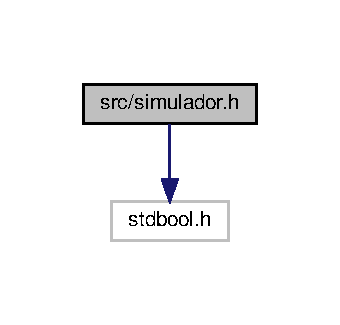
\includegraphics[width=163pt]{simulador_8h__incl}
\end{center}
\end{figure}
This graph shows which files directly or indirectly include this file\+:
\nopagebreak
\begin{figure}[H]
\begin{center}
\leavevmode
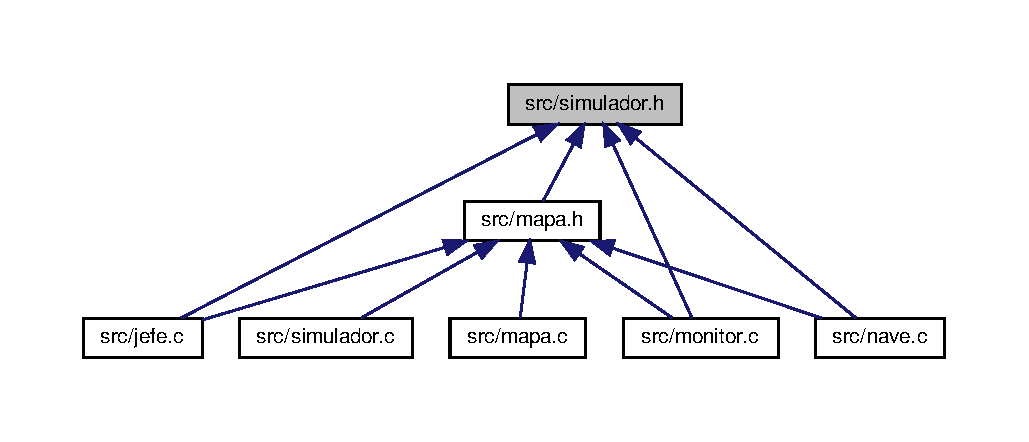
\includegraphics[width=350pt]{simulador_8h__dep__incl}
\end{center}
\end{figure}
\subsection*{Classes}
\begin{DoxyCompactItemize}
\item 
struct \hyperlink{structMensaje}{Mensaje}
\begin{DoxyCompactList}\small\item\em Estructura que almacena los campos necesarios para gestionar los mensajes entre naves y simulador, enviados a traves de cola de mensajes desde las naves. En el mensaje se almacenan la accion a realizar por la nave y sus coordenadas de origen y destino en caso de movimiento, o las coordenadas del atacante y el objetivo en caso de ataque. \end{DoxyCompactList}\item 
struct \hyperlink{structOrden}{Orden}
\begin{DoxyCompactList}\small\item\em Estructura que almacena los campos necesarios para gestionar los mensajes entre el simulador y los jefes, que incluye la orden que realizara el jefe y la nave destinataria en caso de que sea D\+E\+S\+T\+R\+U\+IR. \end{DoxyCompactList}\item 
struct \hyperlink{structtipo__nave}{tipo\+\_\+nave}
\begin{DoxyCompactList}\small\item\em Estructura que almacena la informacion sobre una nave. \end{DoxyCompactList}\item 
struct \hyperlink{structtipo__casilla}{tipo\+\_\+casilla}
\begin{DoxyCompactList}\small\item\em Estructura que almacena la informacion sobre una casilla del mapa. \end{DoxyCompactList}\item 
struct \hyperlink{structtipo__mapa}{tipo\+\_\+mapa}
\begin{DoxyCompactList}\small\item\em Estructura que almacena la informacion sobre el mapa. La estructura original proporcionada ha sido modificada para incluir un contador de los mensajes leidos y enviados por la cola de mensajes, y de los equipos que se vayan quedando sin naves. Esto facilita la reutilizacion de la zona de memoria compartida para el mapa, que permite utilizar estos nuevos campos sin necesidad de crear mas memoria compartida. \end{DoxyCompactList}\item 
struct \hyperlink{structTuberia}{Tuberia}
\begin{DoxyCompactList}\small\item\em Estructura que almacena tantos descriptores de ficheros como naves y jefes haya en la aplicacion. Se utilizara para inicializar las tuberias. \end{DoxyCompactList}\end{DoxyCompactItemize}
\subsection*{Macros}
\begin{DoxyCompactItemize}
\item 
\#define \hyperlink{simulador_8h_ab306668933fb4316ac0f5ef291d13dff}{N\+\_\+\+E\+Q\+U\+I\+P\+OS}~3
\item 
\#define \hyperlink{simulador_8h_aa1f2aba814c6d46772f9694849eeaa7a}{N\+\_\+\+N\+A\+V\+ES}~3
\item 
\#define \hyperlink{simulador_8h_ab55303c06ac5e3f77559983df0288e73}{M\+A\+P\+A\+\_\+\+M\+A\+XX}~10
\item 
\#define \hyperlink{simulador_8h_a5ae04aabcd69e10042a64a5dcf9a959d}{M\+A\+P\+A\+\_\+\+M\+A\+XY}~10
\item 
\#define \hyperlink{simulador_8h_ae58c99716cdc7367c33370378abc028e}{S\+C\+R\+E\+E\+N\+\_\+\+R\+E\+F\+R\+E\+SH}~10000
\item 
\#define \hyperlink{simulador_8h_adb88bdcd56a92b317684f760ff8e45ea}{S\+Y\+M\+B\+\_\+\+V\+A\+C\+IO}~\textquotesingle{}.\textquotesingle{}
\item 
\#define \hyperlink{simulador_8h_acbaa4801c729e0d091227d4f64a51c9c}{S\+Y\+M\+B\+\_\+\+T\+O\+C\+A\+DO}~\textquotesingle{}\%\textquotesingle{}
\item 
\#define \hyperlink{simulador_8h_a9b71befc279d8c06f47141227e7e6da9}{S\+Y\+M\+B\+\_\+\+D\+E\+S\+T\+R\+U\+I\+DO}~\textquotesingle{}X\textquotesingle{}
\item 
\#define \hyperlink{simulador_8h_a8335c476ccea82eea1ba65a7f64afe6b}{S\+Y\+M\+B\+\_\+\+A\+G\+UA}~\textquotesingle{}w\textquotesingle{}
\item 
\#define \hyperlink{simulador_8h_ade0a06566eb0ebcdbbd6cad6e1bd4f2b}{V\+I\+D\+A\+\_\+\+M\+AX}~5
\item 
\#define \hyperlink{simulador_8h_ade0024218fd0d3e02f81dfbbb85a3441}{A\+T\+A\+Q\+U\+E\+\_\+\+A\+L\+C\+A\+N\+CE}~8
\item 
\#define \hyperlink{simulador_8h_a07b6ef9952b43fc051ae7ec4ed494fd3}{A\+T\+A\+Q\+U\+E\+\_\+\+D\+A\+NO}~10
\item 
\#define \hyperlink{simulador_8h_af4b46b99642c235999d1137de80c70eb}{M\+O\+V\+E\+R\+\_\+\+A\+L\+C\+A\+N\+CE}~1
\item 
\#define \hyperlink{simulador_8h_a4f57e1217f555fee4251f319799b9bff}{T\+U\+R\+N\+O\+\_\+\+S\+E\+CS}~5
\item 
\#define \hyperlink{simulador_8h_a9b156bcbd78f59181b3fe0de819d6a0c}{S\+H\+M\+\_\+\+M\+A\+P\+\_\+\+N\+A\+ME}~\char`\"{}/shm\+\_\+naves\char`\"{}
\end{DoxyCompactItemize}
\subsection*{Enumerations}
\begin{DoxyCompactItemize}
\item 
enum \hyperlink{simulador_8h_abddf580b360dbb86fa351f5a944ff315}{Accion} \{ \newline
\hyperlink{simulador_8h_abddf580b360dbb86fa351f5a944ff315adde90091ab8f3559e4c7c923fde07693}{T\+U\+R\+NO}, 
\hyperlink{simulador_8h_abddf580b360dbb86fa351f5a944ff315ab8b0bab740a6d326700455bb8ab25523}{A\+T\+A\+C\+AR}, 
\hyperlink{simulador_8h_abddf580b360dbb86fa351f5a944ff315aea3c073df31939c172972ef6ccbc988b}{F\+IN}, 
\hyperlink{simulador_8h_abddf580b360dbb86fa351f5a944ff315abbd73f1677fcff45aadef7ad7d1c6b80}{M\+O\+V\+ER}, 
\newline
\hyperlink{simulador_8h_abddf580b360dbb86fa351f5a944ff315a363e0d9905ed7c2e02c2f65430aee3c9}{D\+E\+S\+T\+R\+U\+IR}
 \}\begin{DoxyCompactList}\small\item\em enumarado con las posibles acciones que se enviaran a los jefes, a las naves y al simulador. \end{DoxyCompactList}
\end{DoxyCompactItemize}
\subsection*{Variables}
\begin{DoxyCompactItemize}
\item 
char \hyperlink{simulador_8h_a8aa1e6a79521de10e22a0a7574f2c8a5}{symbol\+\_\+equipos} \mbox{[}\hyperlink{simulador_8h_ab306668933fb4316ac0f5ef291d13dff}{N\+\_\+\+E\+Q\+U\+I\+P\+OS}\mbox{]}
\end{DoxyCompactItemize}


\subsection{Detailed Description}
Libreria que contiene todas las constantes, tipos de datos y estructuras manejadas por la aplicacion. 

\begin{DoxyAuthor}{Author}
Alba Ramos\+: \href{mailto:alba.ramosp@estudiante.uam.es}{\tt alba.\+ramosp@estudiante.\+uam.\+es}; Grupo 2213 

Andrea Salcedo\+: \href{mailto:andrea.salcedo@estudiante.uam.es}{\tt andrea.\+salcedo@estudiante.\+uam.\+es}; Grupo 2213 
\end{DoxyAuthor}
\begin{DoxyDate}{Date}
11-\/04-\/2019 
\end{DoxyDate}


\subsection{Macro Definition Documentation}
\mbox{\Hypertarget{simulador_8h_ade0024218fd0d3e02f81dfbbb85a3441}\label{simulador_8h_ade0024218fd0d3e02f81dfbbb85a3441}} 
\index{simulador.\+h@{simulador.\+h}!A\+T\+A\+Q\+U\+E\+\_\+\+A\+L\+C\+A\+N\+CE@{A\+T\+A\+Q\+U\+E\+\_\+\+A\+L\+C\+A\+N\+CE}}
\index{A\+T\+A\+Q\+U\+E\+\_\+\+A\+L\+C\+A\+N\+CE@{A\+T\+A\+Q\+U\+E\+\_\+\+A\+L\+C\+A\+N\+CE}!simulador.\+h@{simulador.\+h}}
\subsubsection{\texorpdfstring{A\+T\+A\+Q\+U\+E\+\_\+\+A\+L\+C\+A\+N\+CE}{ATAQUE\_ALCANCE}}
{\footnotesize\ttfamily \#define A\+T\+A\+Q\+U\+E\+\_\+\+A\+L\+C\+A\+N\+CE~8}

Distancia máxima de un ataque \mbox{\Hypertarget{simulador_8h_a07b6ef9952b43fc051ae7ec4ed494fd3}\label{simulador_8h_a07b6ef9952b43fc051ae7ec4ed494fd3}} 
\index{simulador.\+h@{simulador.\+h}!A\+T\+A\+Q\+U\+E\+\_\+\+D\+A\+NO@{A\+T\+A\+Q\+U\+E\+\_\+\+D\+A\+NO}}
\index{A\+T\+A\+Q\+U\+E\+\_\+\+D\+A\+NO@{A\+T\+A\+Q\+U\+E\+\_\+\+D\+A\+NO}!simulador.\+h@{simulador.\+h}}
\subsubsection{\texorpdfstring{A\+T\+A\+Q\+U\+E\+\_\+\+D\+A\+NO}{ATAQUE\_DANO}}
{\footnotesize\ttfamily \#define A\+T\+A\+Q\+U\+E\+\_\+\+D\+A\+NO~10}

Daño de un ataque \mbox{\Hypertarget{simulador_8h_ab55303c06ac5e3f77559983df0288e73}\label{simulador_8h_ab55303c06ac5e3f77559983df0288e73}} 
\index{simulador.\+h@{simulador.\+h}!M\+A\+P\+A\+\_\+\+M\+A\+XX@{M\+A\+P\+A\+\_\+\+M\+A\+XX}}
\index{M\+A\+P\+A\+\_\+\+M\+A\+XX@{M\+A\+P\+A\+\_\+\+M\+A\+XX}!simulador.\+h@{simulador.\+h}}
\subsubsection{\texorpdfstring{M\+A\+P\+A\+\_\+\+M\+A\+XX}{MAPA\_MAXX}}
{\footnotesize\ttfamily \#define M\+A\+P\+A\+\_\+\+M\+A\+XX~10}

Número de columnas del mapa \mbox{\Hypertarget{simulador_8h_a5ae04aabcd69e10042a64a5dcf9a959d}\label{simulador_8h_a5ae04aabcd69e10042a64a5dcf9a959d}} 
\index{simulador.\+h@{simulador.\+h}!M\+A\+P\+A\+\_\+\+M\+A\+XY@{M\+A\+P\+A\+\_\+\+M\+A\+XY}}
\index{M\+A\+P\+A\+\_\+\+M\+A\+XY@{M\+A\+P\+A\+\_\+\+M\+A\+XY}!simulador.\+h@{simulador.\+h}}
\subsubsection{\texorpdfstring{M\+A\+P\+A\+\_\+\+M\+A\+XY}{MAPA\_MAXY}}
{\footnotesize\ttfamily \#define M\+A\+P\+A\+\_\+\+M\+A\+XY~10}

Número de filas del mapa \mbox{\Hypertarget{simulador_8h_af4b46b99642c235999d1137de80c70eb}\label{simulador_8h_af4b46b99642c235999d1137de80c70eb}} 
\index{simulador.\+h@{simulador.\+h}!M\+O\+V\+E\+R\+\_\+\+A\+L\+C\+A\+N\+CE@{M\+O\+V\+E\+R\+\_\+\+A\+L\+C\+A\+N\+CE}}
\index{M\+O\+V\+E\+R\+\_\+\+A\+L\+C\+A\+N\+CE@{M\+O\+V\+E\+R\+\_\+\+A\+L\+C\+A\+N\+CE}!simulador.\+h@{simulador.\+h}}
\subsubsection{\texorpdfstring{M\+O\+V\+E\+R\+\_\+\+A\+L\+C\+A\+N\+CE}{MOVER\_ALCANCE}}
{\footnotesize\ttfamily \#define M\+O\+V\+E\+R\+\_\+\+A\+L\+C\+A\+N\+CE~1}

Máximo de casillas a mover \mbox{\Hypertarget{simulador_8h_ab306668933fb4316ac0f5ef291d13dff}\label{simulador_8h_ab306668933fb4316ac0f5ef291d13dff}} 
\index{simulador.\+h@{simulador.\+h}!N\+\_\+\+E\+Q\+U\+I\+P\+OS@{N\+\_\+\+E\+Q\+U\+I\+P\+OS}}
\index{N\+\_\+\+E\+Q\+U\+I\+P\+OS@{N\+\_\+\+E\+Q\+U\+I\+P\+OS}!simulador.\+h@{simulador.\+h}}
\subsubsection{\texorpdfstring{N\+\_\+\+E\+Q\+U\+I\+P\+OS}{N\_EQUIPOS}}
{\footnotesize\ttfamily \#define N\+\_\+\+E\+Q\+U\+I\+P\+OS~3}

Número de equipos \mbox{\Hypertarget{simulador_8h_aa1f2aba814c6d46772f9694849eeaa7a}\label{simulador_8h_aa1f2aba814c6d46772f9694849eeaa7a}} 
\index{simulador.\+h@{simulador.\+h}!N\+\_\+\+N\+A\+V\+ES@{N\+\_\+\+N\+A\+V\+ES}}
\index{N\+\_\+\+N\+A\+V\+ES@{N\+\_\+\+N\+A\+V\+ES}!simulador.\+h@{simulador.\+h}}
\subsubsection{\texorpdfstring{N\+\_\+\+N\+A\+V\+ES}{N\_NAVES}}
{\footnotesize\ttfamily \#define N\+\_\+\+N\+A\+V\+ES~3}

Número de naves por equipo \mbox{\Hypertarget{simulador_8h_ae58c99716cdc7367c33370378abc028e}\label{simulador_8h_ae58c99716cdc7367c33370378abc028e}} 
\index{simulador.\+h@{simulador.\+h}!S\+C\+R\+E\+E\+N\+\_\+\+R\+E\+F\+R\+E\+SH@{S\+C\+R\+E\+E\+N\+\_\+\+R\+E\+F\+R\+E\+SH}}
\index{S\+C\+R\+E\+E\+N\+\_\+\+R\+E\+F\+R\+E\+SH@{S\+C\+R\+E\+E\+N\+\_\+\+R\+E\+F\+R\+E\+SH}!simulador.\+h@{simulador.\+h}}
\subsubsection{\texorpdfstring{S\+C\+R\+E\+E\+N\+\_\+\+R\+E\+F\+R\+E\+SH}{SCREEN\_REFRESH}}
{\footnotesize\ttfamily \#define S\+C\+R\+E\+E\+N\+\_\+\+R\+E\+F\+R\+E\+SH~10000}

Frequencia de refresco del mapa en el monitor \mbox{\Hypertarget{simulador_8h_a9b156bcbd78f59181b3fe0de819d6a0c}\label{simulador_8h_a9b156bcbd78f59181b3fe0de819d6a0c}} 
\index{simulador.\+h@{simulador.\+h}!S\+H\+M\+\_\+\+M\+A\+P\+\_\+\+N\+A\+ME@{S\+H\+M\+\_\+\+M\+A\+P\+\_\+\+N\+A\+ME}}
\index{S\+H\+M\+\_\+\+M\+A\+P\+\_\+\+N\+A\+ME@{S\+H\+M\+\_\+\+M\+A\+P\+\_\+\+N\+A\+ME}!simulador.\+h@{simulador.\+h}}
\subsubsection{\texorpdfstring{S\+H\+M\+\_\+\+M\+A\+P\+\_\+\+N\+A\+ME}{SHM\_MAP\_NAME}}
{\footnotesize\ttfamily \#define S\+H\+M\+\_\+\+M\+A\+P\+\_\+\+N\+A\+ME~\char`\"{}/shm\+\_\+naves\char`\"{}}

\mbox{\Hypertarget{simulador_8h_a8335c476ccea82eea1ba65a7f64afe6b}\label{simulador_8h_a8335c476ccea82eea1ba65a7f64afe6b}} 
\index{simulador.\+h@{simulador.\+h}!S\+Y\+M\+B\+\_\+\+A\+G\+UA@{S\+Y\+M\+B\+\_\+\+A\+G\+UA}}
\index{S\+Y\+M\+B\+\_\+\+A\+G\+UA@{S\+Y\+M\+B\+\_\+\+A\+G\+UA}!simulador.\+h@{simulador.\+h}}
\subsubsection{\texorpdfstring{S\+Y\+M\+B\+\_\+\+A\+G\+UA}{SYMB\_AGUA}}
{\footnotesize\ttfamily \#define S\+Y\+M\+B\+\_\+\+A\+G\+UA~\textquotesingle{}w\textquotesingle{}}

Símbolo para agua \mbox{\Hypertarget{simulador_8h_a9b71befc279d8c06f47141227e7e6da9}\label{simulador_8h_a9b71befc279d8c06f47141227e7e6da9}} 
\index{simulador.\+h@{simulador.\+h}!S\+Y\+M\+B\+\_\+\+D\+E\+S\+T\+R\+U\+I\+DO@{S\+Y\+M\+B\+\_\+\+D\+E\+S\+T\+R\+U\+I\+DO}}
\index{S\+Y\+M\+B\+\_\+\+D\+E\+S\+T\+R\+U\+I\+DO@{S\+Y\+M\+B\+\_\+\+D\+E\+S\+T\+R\+U\+I\+DO}!simulador.\+h@{simulador.\+h}}
\subsubsection{\texorpdfstring{S\+Y\+M\+B\+\_\+\+D\+E\+S\+T\+R\+U\+I\+DO}{SYMB\_DESTRUIDO}}
{\footnotesize\ttfamily \#define S\+Y\+M\+B\+\_\+\+D\+E\+S\+T\+R\+U\+I\+DO~\textquotesingle{}X\textquotesingle{}}

Símbolo para destruido \mbox{\Hypertarget{simulador_8h_acbaa4801c729e0d091227d4f64a51c9c}\label{simulador_8h_acbaa4801c729e0d091227d4f64a51c9c}} 
\index{simulador.\+h@{simulador.\+h}!S\+Y\+M\+B\+\_\+\+T\+O\+C\+A\+DO@{S\+Y\+M\+B\+\_\+\+T\+O\+C\+A\+DO}}
\index{S\+Y\+M\+B\+\_\+\+T\+O\+C\+A\+DO@{S\+Y\+M\+B\+\_\+\+T\+O\+C\+A\+DO}!simulador.\+h@{simulador.\+h}}
\subsubsection{\texorpdfstring{S\+Y\+M\+B\+\_\+\+T\+O\+C\+A\+DO}{SYMB\_TOCADO}}
{\footnotesize\ttfamily \#define S\+Y\+M\+B\+\_\+\+T\+O\+C\+A\+DO~\textquotesingle{}\%\textquotesingle{}}

Símbolo para tocado \mbox{\Hypertarget{simulador_8h_adb88bdcd56a92b317684f760ff8e45ea}\label{simulador_8h_adb88bdcd56a92b317684f760ff8e45ea}} 
\index{simulador.\+h@{simulador.\+h}!S\+Y\+M\+B\+\_\+\+V\+A\+C\+IO@{S\+Y\+M\+B\+\_\+\+V\+A\+C\+IO}}
\index{S\+Y\+M\+B\+\_\+\+V\+A\+C\+IO@{S\+Y\+M\+B\+\_\+\+V\+A\+C\+IO}!simulador.\+h@{simulador.\+h}}
\subsubsection{\texorpdfstring{S\+Y\+M\+B\+\_\+\+V\+A\+C\+IO}{SYMB\_VACIO}}
{\footnotesize\ttfamily \#define S\+Y\+M\+B\+\_\+\+V\+A\+C\+IO~\textquotesingle{}.\textquotesingle{}}

Símbolo para casilla vacia \mbox{\Hypertarget{simulador_8h_a4f57e1217f555fee4251f319799b9bff}\label{simulador_8h_a4f57e1217f555fee4251f319799b9bff}} 
\index{simulador.\+h@{simulador.\+h}!T\+U\+R\+N\+O\+\_\+\+S\+E\+CS@{T\+U\+R\+N\+O\+\_\+\+S\+E\+CS}}
\index{T\+U\+R\+N\+O\+\_\+\+S\+E\+CS@{T\+U\+R\+N\+O\+\_\+\+S\+E\+CS}!simulador.\+h@{simulador.\+h}}
\subsubsection{\texorpdfstring{T\+U\+R\+N\+O\+\_\+\+S\+E\+CS}{TURNO\_SECS}}
{\footnotesize\ttfamily \#define T\+U\+R\+N\+O\+\_\+\+S\+E\+CS~5}

Segundos que dura un turno \mbox{\Hypertarget{simulador_8h_ade0a06566eb0ebcdbbd6cad6e1bd4f2b}\label{simulador_8h_ade0a06566eb0ebcdbbd6cad6e1bd4f2b}} 
\index{simulador.\+h@{simulador.\+h}!V\+I\+D\+A\+\_\+\+M\+AX@{V\+I\+D\+A\+\_\+\+M\+AX}}
\index{V\+I\+D\+A\+\_\+\+M\+AX@{V\+I\+D\+A\+\_\+\+M\+AX}!simulador.\+h@{simulador.\+h}}
\subsubsection{\texorpdfstring{V\+I\+D\+A\+\_\+\+M\+AX}{VIDA\_MAX}}
{\footnotesize\ttfamily \#define V\+I\+D\+A\+\_\+\+M\+AX~5}

Vida inicial de una nave 

\subsection{Enumeration Type Documentation}
\mbox{\Hypertarget{simulador_8h_abddf580b360dbb86fa351f5a944ff315}\label{simulador_8h_abddf580b360dbb86fa351f5a944ff315}} 
\index{simulador.\+h@{simulador.\+h}!Accion@{Accion}}
\index{Accion@{Accion}!simulador.\+h@{simulador.\+h}}
\subsubsection{\texorpdfstring{Accion}{Accion}}
{\footnotesize\ttfamily enum \hyperlink{simulador_8h_abddf580b360dbb86fa351f5a944ff315}{Accion}}



enumarado con las posibles acciones que se enviaran a los jefes, a las naves y al simulador. 

\begin{DoxyEnumFields}{Enumerator}
\raisebox{\heightof{T}}[0pt][0pt]{\index{T\+U\+R\+NO@{T\+U\+R\+NO}!simulador.\+h@{simulador.\+h}}\index{simulador.\+h@{simulador.\+h}!T\+U\+R\+NO@{T\+U\+R\+NO}}}\mbox{\Hypertarget{simulador_8h_abddf580b360dbb86fa351f5a944ff315adde90091ab8f3559e4c7c923fde07693}\label{simulador_8h_abddf580b360dbb86fa351f5a944ff315adde90091ab8f3559e4c7c923fde07693}} 
T\+U\+R\+NO&\\
\hline

\raisebox{\heightof{T}}[0pt][0pt]{\index{A\+T\+A\+C\+AR@{A\+T\+A\+C\+AR}!simulador.\+h@{simulador.\+h}}\index{simulador.\+h@{simulador.\+h}!A\+T\+A\+C\+AR@{A\+T\+A\+C\+AR}}}\mbox{\Hypertarget{simulador_8h_abddf580b360dbb86fa351f5a944ff315ab8b0bab740a6d326700455bb8ab25523}\label{simulador_8h_abddf580b360dbb86fa351f5a944ff315ab8b0bab740a6d326700455bb8ab25523}} 
A\+T\+A\+C\+AR&\\
\hline

\raisebox{\heightof{T}}[0pt][0pt]{\index{F\+IN@{F\+IN}!simulador.\+h@{simulador.\+h}}\index{simulador.\+h@{simulador.\+h}!F\+IN@{F\+IN}}}\mbox{\Hypertarget{simulador_8h_abddf580b360dbb86fa351f5a944ff315aea3c073df31939c172972ef6ccbc988b}\label{simulador_8h_abddf580b360dbb86fa351f5a944ff315aea3c073df31939c172972ef6ccbc988b}} 
F\+IN&\\
\hline

\raisebox{\heightof{T}}[0pt][0pt]{\index{M\+O\+V\+ER@{M\+O\+V\+ER}!simulador.\+h@{simulador.\+h}}\index{simulador.\+h@{simulador.\+h}!M\+O\+V\+ER@{M\+O\+V\+ER}}}\mbox{\Hypertarget{simulador_8h_abddf580b360dbb86fa351f5a944ff315abbd73f1677fcff45aadef7ad7d1c6b80}\label{simulador_8h_abddf580b360dbb86fa351f5a944ff315abbd73f1677fcff45aadef7ad7d1c6b80}} 
M\+O\+V\+ER&\\
\hline

\raisebox{\heightof{T}}[0pt][0pt]{\index{D\+E\+S\+T\+R\+U\+IR@{D\+E\+S\+T\+R\+U\+IR}!simulador.\+h@{simulador.\+h}}\index{simulador.\+h@{simulador.\+h}!D\+E\+S\+T\+R\+U\+IR@{D\+E\+S\+T\+R\+U\+IR}}}\mbox{\Hypertarget{simulador_8h_abddf580b360dbb86fa351f5a944ff315a363e0d9905ed7c2e02c2f65430aee3c9}\label{simulador_8h_abddf580b360dbb86fa351f5a944ff315a363e0d9905ed7c2e02c2f65430aee3c9}} 
D\+E\+S\+T\+R\+U\+IR&\\
\hline

\end{DoxyEnumFields}


\subsection{Variable Documentation}
\mbox{\Hypertarget{simulador_8h_a8aa1e6a79521de10e22a0a7574f2c8a5}\label{simulador_8h_a8aa1e6a79521de10e22a0a7574f2c8a5}} 
\index{simulador.\+h@{simulador.\+h}!symbol\+\_\+equipos@{symbol\+\_\+equipos}}
\index{symbol\+\_\+equipos@{symbol\+\_\+equipos}!simulador.\+h@{simulador.\+h}}
\subsubsection{\texorpdfstring{symbol\+\_\+equipos}{symbol\_equipos}}
{\footnotesize\ttfamily char symbol\+\_\+equipos\mbox{[}\hyperlink{simulador_8h_ab306668933fb4316ac0f5ef291d13dff}{N\+\_\+\+E\+Q\+U\+I\+P\+OS}\mbox{]}}

Símbolos de los diferentes equipos en el mapa (mirar \hyperlink{mapa_8c}{mapa.\+c}) 
%--- End generated contents ---

% Index
\backmatter
\newpage
\phantomsection
\clearemptydoublepage
\addcontentsline{toc}{chapter}{Index}
\printindex

\end{document}
